\documentclass[paper=a4, fontsize=11pt]{report}
\usepackage{mathtools}
\usepackage[a4paper,bindingoffset=0.2in,%
            left=1in,right=1in,top=1in,bottom=1in,%
            footskip=.5in]{geometry}
\usepackage{listings}
\usepackage{color}
\definecolor{darkred}{rgb}{0.26,0.23,0.23}
\lstset{language=TeX, basicstyle=\ttfamily\color{darkred}, keywordstyle=\ttfamily\color{darkred}, emphstyle=\itshape, emph={options}, commentstyle=\itshape, lineskip=0pt} 




\usepackage{Sweave}
\begin{document}
\Sconcordance{concordance:PreReport.tex:PreReport.Rnw:%
1 7 1 1 0 7 1 1 5 10 1 1 6 1 0 4 1 3 0 1 2 10 1 1 2 16 0 1 2 1 4 3 1 1 %
10 2 0 1 2 4 0 1 5 9 1 1 6 1 0 3 1 3 0 1 5 29 1 1 5 1 3 2 0 2 1 5 0 1 1 %
5 0 1 1 5 0 1 1 6 0 1 2 1 4 15 1 1 7 1 0 3 1 1 2 4 0 1 2 10 1 1 2 1 0 1 %
1 1 2 6 0 1 2 6 0 1 2 13 0 1 5 7 1 1 2 1 0 3 1 6 0 1 2 4 1 1 2 1 0 1 1 %
5 0 1 1 6 0 1 2 1 1 1 2 1 0 1 1 1 2 1 0 1 1 6 0 1 2 1 1 1 70 27 1 1 6 1 %
4 3 0 1 1 3 0 1 2 1 4 15 1 11 0 1 10 3 1 11 0 1 10 2 1 24 0 1 23 7 1 1 %
6 1 7 1 4 9 1 1 6 1 9 1 4 13 1 1 7 1 0 1 1 1 7 6 0 1 1 1 2 1 1 5 0 1 1 %
5 0 1 1 5 0 1 1 6 0 1 5 11 1 12 0 1 11 5 1 14 0 1 13 17 1 14 0 1 13 5 1 %
1 6 1 0 5 1 3 0 1 5 8 1 1 2 20 0 1 18 30 1 1 7 2 0 4 1 5 0 1 1 6 0 1 5 %
11 1 1 2 1 0 3 1 1 2 1 0 3 1 4 0 1 3 11 1 1 3 2 0 1 2 1 0 1 3 2 0 1 2 4 %
0 1 2 2 1 1 3 2 0 1 1 1 2 1 0 1 2 1 0 1 1 3 0 1 2 35 1}

\setlength{\parindent}{0}
\noindent

\title{Emulate \texttt{persp} plot and \texttt{filled.contour} plot on \texttt{gridGraphics}}
\maketitle
\chapter{Introduction}
\section{Background}
The core graphics system in \texttt{R} can been divided in to two main packages. The first package is the \texttt{graphics} package. It is older and it provides the original GRZ graphics system from \texttt{S}, sometimes referred to as ``traditional'' graphics. It is relatively fast and many other \texttt{R} packages build on top of it. The newer package is the \texttt{grid} package. It is actually slower but is has more flexibility and additional features compared to the \texttt{graphics} package. \\

A graph that is drawn using \texttt{grid} can been edited in many more ways than a graph that has been drawn using the basic \texttt{graphics} package. However, there is a new package, called \texttt{gridGraphics}, which allows us to convert a plot that has been drawn by the \texttt{graphics} package to an equivalent plot drawn by \texttt{grid} graphics. This means that the additional flexibility and features of \texttt{grid} become available for any plot drawn using the \texttt{graphics} package. \\

\section{The \texttt{gridGraphics} package}
\texttt{gridGraphics} is like a 'translator' that translates a plot that has been drawn using the basic \texttt{graphics} package to a plot that has been drawn using the \texttt{grid} package. \\

The \texttt{gridGraphic} package has a main function called \texttt{grid.echo()}, which takes a recorded plot as an argument (or NULL for the current plot of the current graphics device). The \texttt{grid.echo()} replicates the plot using \texttt{grid} so that the user may edit the plot in more ways than they can with the original plot drawn by basic \texttt{graphic} package.\\

The following code provides a quick example. We generate 25 random numbers for x and y. First, we draw a scatter plot using the function \texttt{plot()} from the basic graphics package, then we redraw it using \texttt{grid.echo()} from the \texttt{gridGraphics} package with \texttt{grid}, see Figure \ref{figure_1.1}
\begin{Schunk}
\begin{Sinput}
> set.seed(110)
> x = runif(25)
> y = runif(25)
> plot(x,y, pch = 16)
> grid.echo()
\end{Sinput}
\end{Schunk}

\newpage
\begin{figure}[h]
\begin{center}
  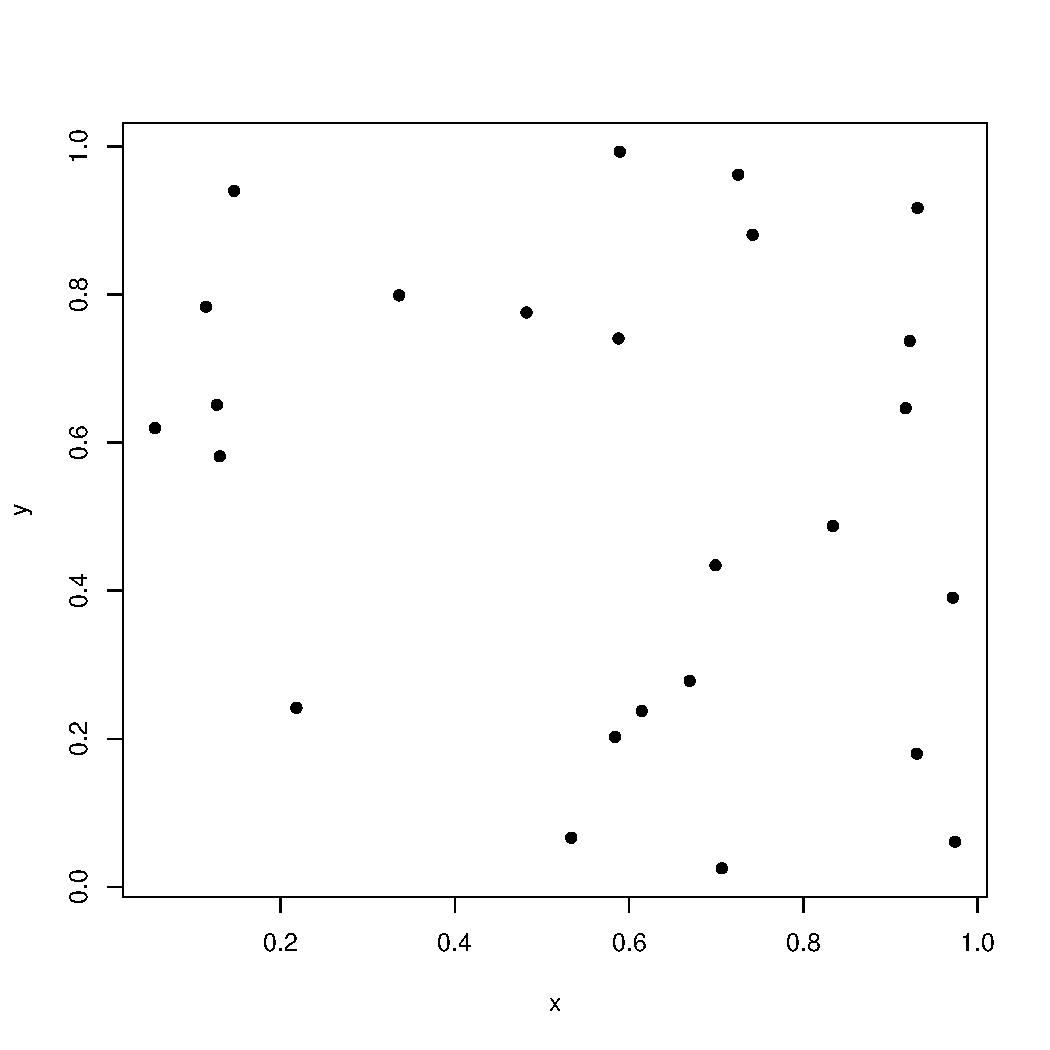
\includegraphics[height = 7.5cm, width = 7.5cm]{figure/report_basic_demo_1.pdf}
  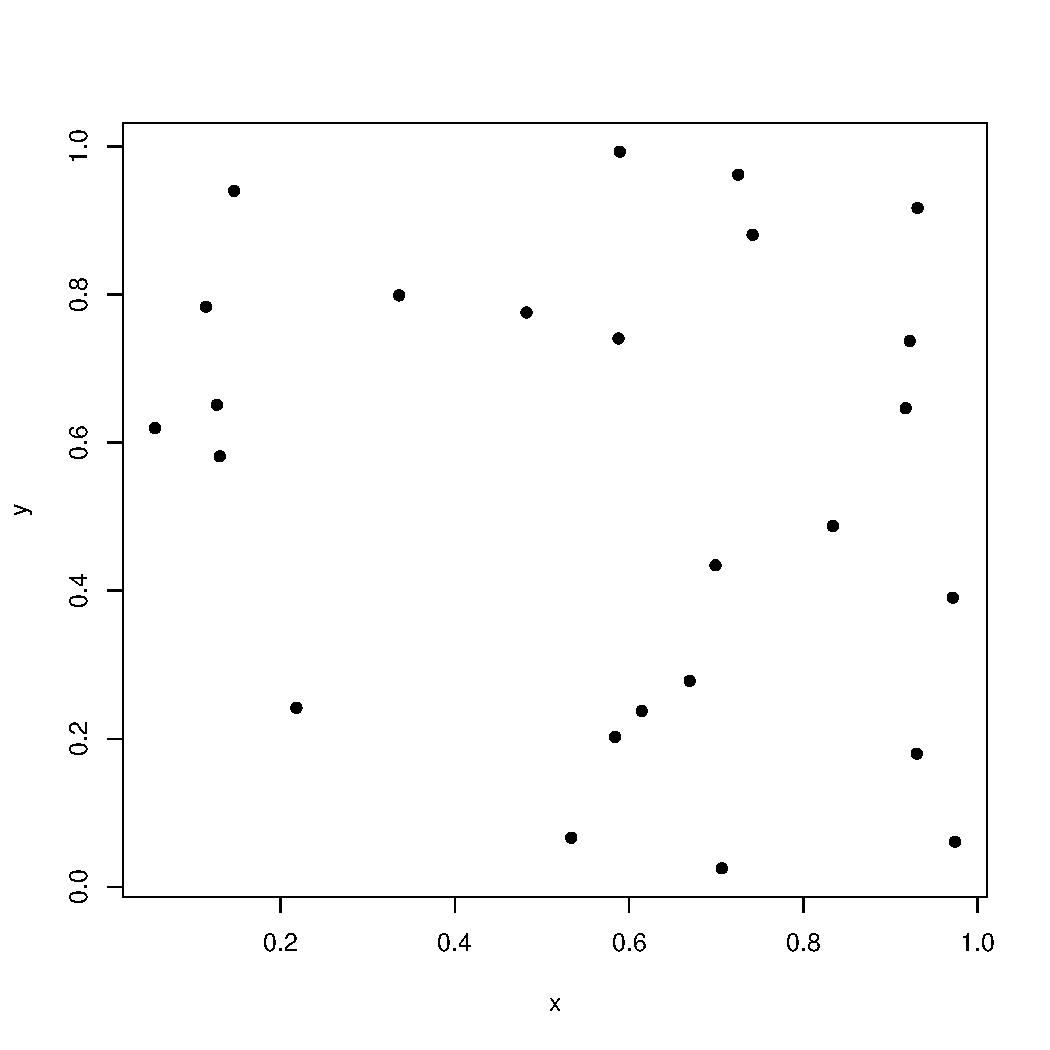
\includegraphics[height = 7.5cm, width = 7.5cm]{figure/report_basic_demo_1.pdf}
  \caption{The left plot is drawn by using \texttt{plot()}; the Right plot is redrawn using \texttt{grid.echo()}. Two plots are identical to each other}
  	\label{figure_1.1}
\end{center}
\end{figure}
One example that shows the advantage of drawing the plot using \texttt{grid} rather than basic \texttt{graphics} is that there are objects, called grid grobs, which recorded a list of the details of each components of the plot that has been drawn. The list of grobs can been seen by calling the function \texttt{grid.ls()}. \\
\begin{Schunk}
\begin{Sinput}
> grid.ls()
\end{Sinput}
\begin{Soutput}
graphics-plot-1-points-1
graphics-plot-1-bottom-axis-line-1
graphics-plot-1-bottom-axis-ticks-1
graphics-plot-1-bottom-axis-labels-1
graphics-plot-1-left-axis-line-1
graphics-plot-1-left-axis-ticks-1
graphics-plot-1-left-axis-labels-1
graphics-plot-1-box-1
graphics-plot-1-xlab-1
graphics-plot-1-ylab-1
\end{Soutput}
\end{Schunk}


As we see, the \texttt{grid.ls()} function returns a list of grid grobs for the previous plot that has been redrawn by \texttt{grid}. There is one element called \textit{graphics-plot-1-bottom-axis-labels-1} which represents the labels of the bottom axis. In \texttt{grid}, there are several functions that can be used to manipulate this grob. See Figure \ref{figure_1.2} \\

For example, if the user wants to rotate the labels of the bottom axis by 30 degrees and changes the color from default to orange, then the following code performs these changes.
\begin{Schunk}
\begin{Sinput}
> grid.edit("graphics-plot-1-bottom-axis-labels-1", 
+           rot=30, gp=gpar(col="orange"))
> grid.edit("graphics-plot-1-left-axis-labels-1", 
+           rot=30, gp=gpar(col="orange"))
\end{Sinput}
\end{Schunk}
\newpage
\begin{figure}[h]
\begin{center}
  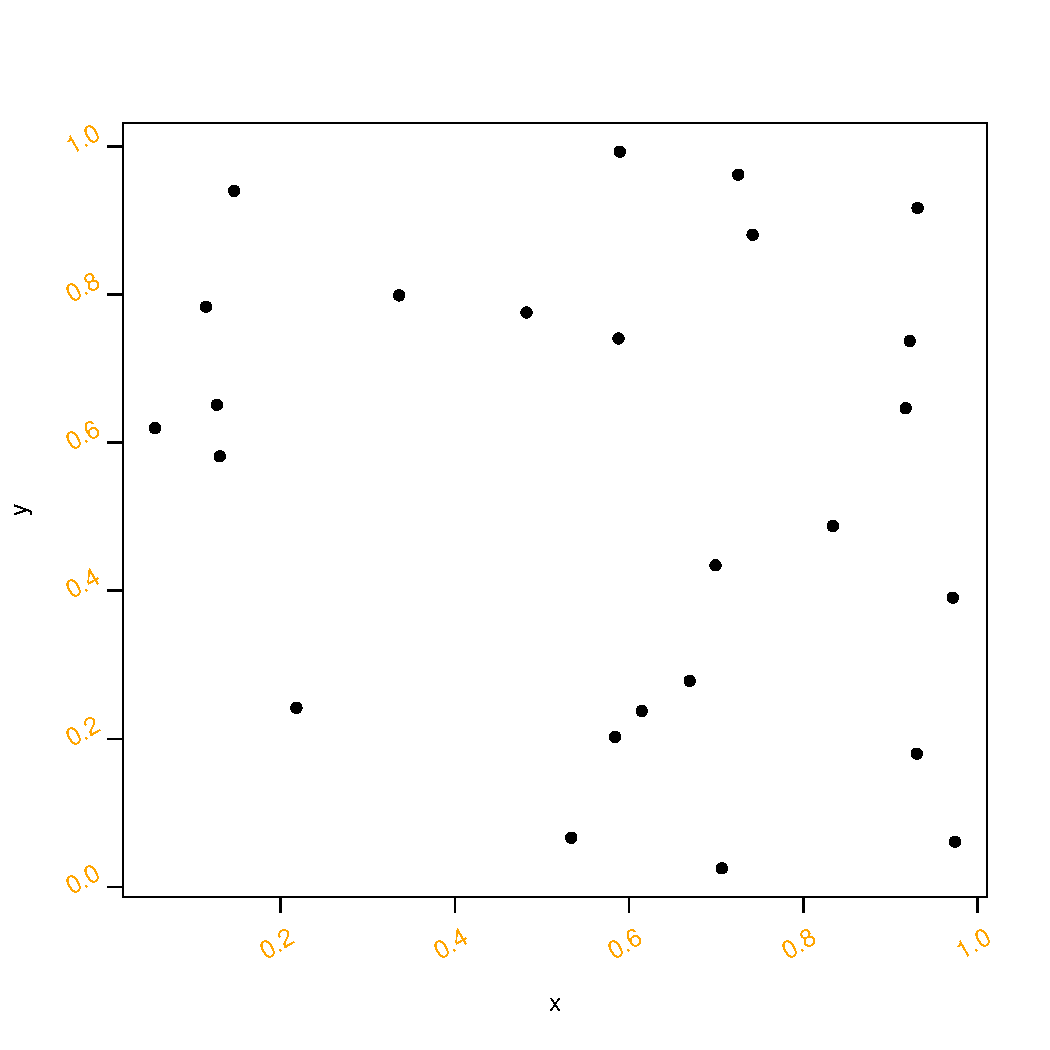
\includegraphics[height = 10cm, width = 10cm]{figure/report_basic_demo_4.pdf}
  \caption{The angle and the color of the bottom and left axis of the previous plot have been changed by 30 degrees and orange}
  	\label{figure_1.2}
\end{center}
\end{figure}
\section{The problem}
The \texttt{grid.echo()} function can replicate most plots that are drawn by the graphics package. However, there are a few functions in the graphics package that \texttt{grid.echo()} cannot replicate. One such function is \texttt{persp()} which draws 3-dimemtional surfaces, the other one is the \texttt{filled.contour()}. If we can draw a plot with \texttt{persp()} or \texttt{filled.countour(),} the result from calling \texttt{grid.echo()} is a (mostly) blank screen. See Figure \ref{figure_1.3}.
\begin{Schunk}
\begin{Sinput}
> x = y = seq(-4*pi, 4*pi, len = 27)
> r = sqrt(outer(x^2, y^2, "+"))
> filled.contour(cos(r^2)*exp(-r/(2*pi)), frame.plot = FALSE, plot.axes = {})
> grid.echo()
\end{Sinput}
\end{Schunk}
\begin{figure}[h]
\begin{center}
  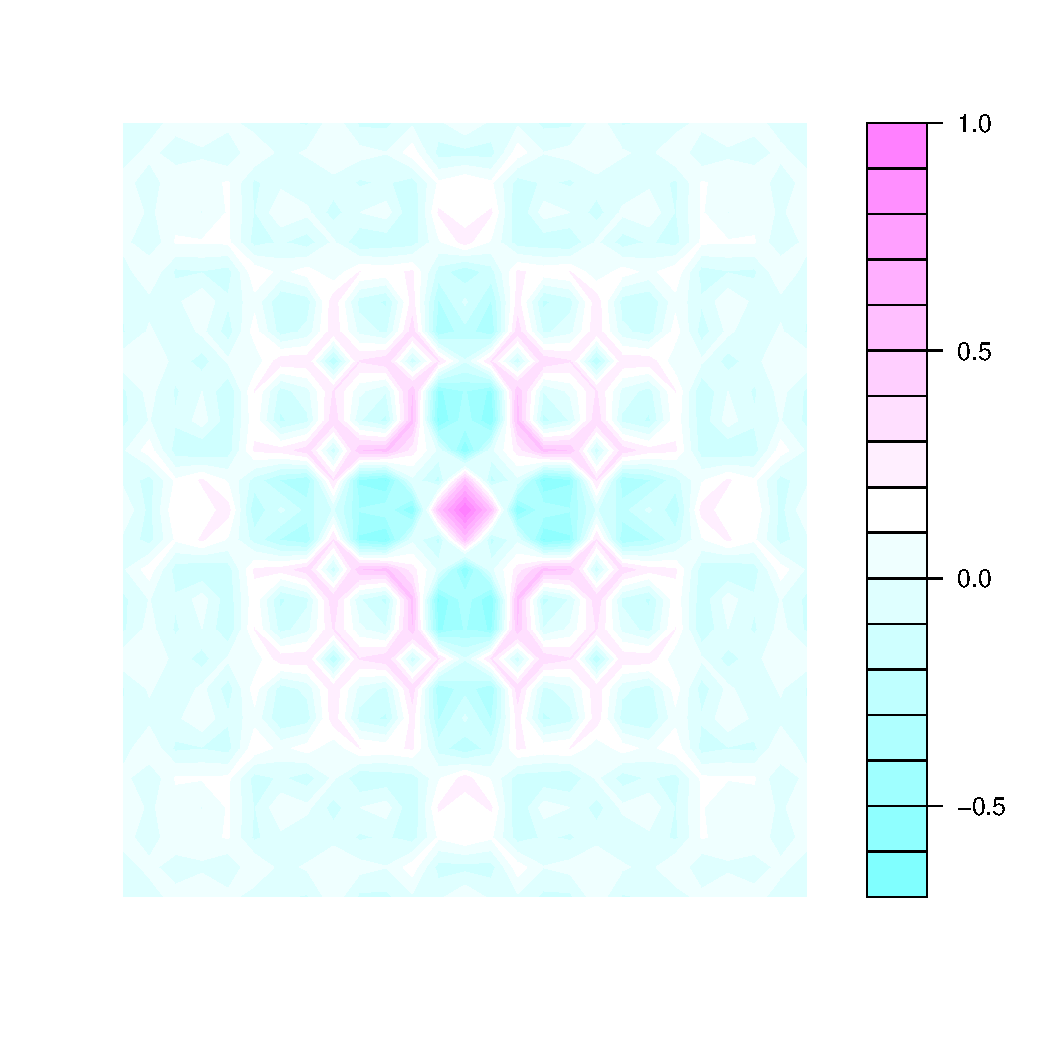
\includegraphics[height = 7.5cm, width = 7.5cm]{figure/report_fill_1}
  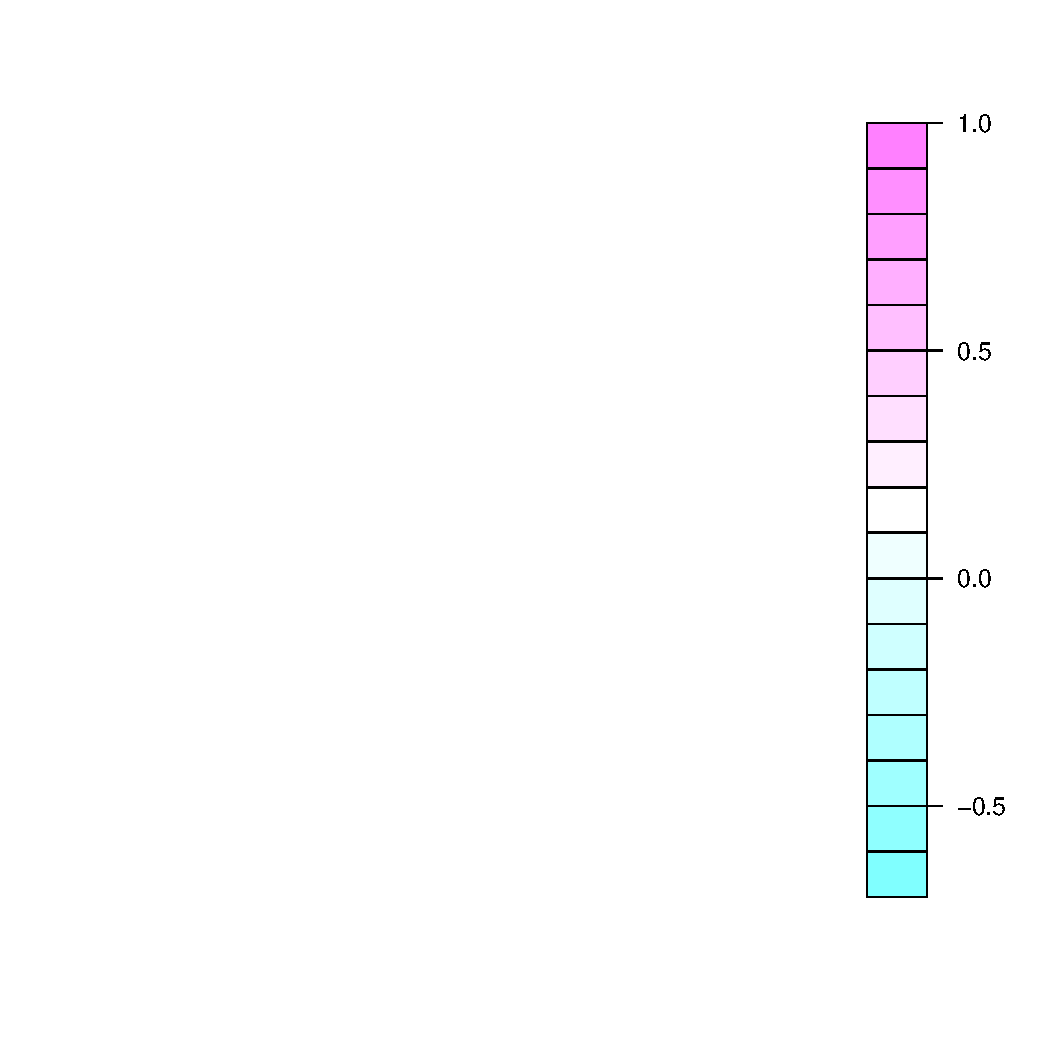
\includegraphics[height = 7.5cm, width = 7.5cm]{figure/report_fill_2}
  \caption{The left plot been drawn by using \texttt{filled.contour()} and the right plot been redrawn by calling \texttt{grid.echo()}. There is a "blank" page on the right plot because the grid.echo cannot emulate \texttt{filled.contour()} in this stage.}
  	\label{figure_1.3}
\end{center}
\end{figure}

\section{Aim of this project}
The purpose of this paper is emulate the Perspective Plots, \texttt{persp()} and Level (Contour) Plots, \texttt{filled.contour()} using the \texttt{grid} package. However, these two functions are written in C, as part of the core \texttt{R} source code. This means that a normal \texttt{R} user or developer cannot modify the code. Also, the \texttt{C} code is structured so that the normal \texttt{R} user or developer cannot separately call the \texttt{C} code. The solution of this paper as follows: 
\newpage
\begin{enumerate}
  \item Emulate the \texttt{persp()} function on \texttt{grid} separate from the \texttt{gridGraphics} package (standalone):
    \begin{enumerate}
      \item Extract the information from the graphics engine display list.
      \item Understanding and translating the calculation that been done by \texttt{C} code from the \texttt{graphics} package to \texttt{R} code
      \item Draw the Perspective Plot on \texttt{grid}.
    \end{enumerate}
  \item integrate the standalone to the \texttt{gridGraphics}
  \color{red}{
    \begin{enumerate}
      \item navigating to the correct viewport that been setted up by \texttt{gridGraphics}
      \item Create a new viewport for setting up the correct x-scale and y-scale preparing for drawing, (if necessary) then draw the contents in the correct viewport.
      \item Test the difference of the plots that been drawn by \texttt{graphics} and \texttt{grid}
    \end{enumerate}
  }
\end{enumerate}



% NOTE to Jason: explain how gridGraphics works first: graphics display list; gridGraphics implements an R version of each low-level C function on the display list (e.g., for C\_plot\_xy there is an R function called C\_plot\_xy in the gridGraphics package). THEN maybe write about 3D to 2D transformations, but only maybe.% 


\chapter{The graphics engine display list}
The information for every plot drawn by R can be recorded. For example, In the simple \texttt{plot()} function, it is possible to obtain the parameters for x and y, even the label of the x-axis and y-axis. See Figure\ref{figure_2.1}.\\

This information is called the graphics engine display list. In this paper, we use this graphics engine display list to replicate the \texttt{persp()} plot and \texttt{filled.contour()} plot using grid. The \texttt{recordPlot()} function can be used to access the graphics engine display list, the \texttt{recordPlot()} function been used. This function saves the plot in an R object. 

\begin{Schunk}
\begin{Sinput}
> plot(cars$speed, cars$dist, col = 'orange', 
+       pch = 16, xlab = 'speed', ylab = 'dist')
> reco = recordPlot()[[1]][[4]][[2]][[2]]
> head(reco[[1]]) #x
\end{Sinput}
\begin{Soutput}
[1] 4 4 7 7 8 9
\end{Soutput}
\begin{Sinput}
> head(reco[[2]]) #y
\end{Sinput}
\begin{Soutput}
[1]  2 10  4 22 16 10
\end{Soutput}
\begin{Sinput}
> reco$xlab
\end{Sinput}
\begin{Soutput}
[1] "cars$speed"
\end{Soutput}
\begin{Sinput}
> reco$ylab
\end{Sinput}
\begin{Soutput}
[1] "cars$dist"
\end{Soutput}
\end{Schunk}


\begin{figure}[h]
\begin{center}
  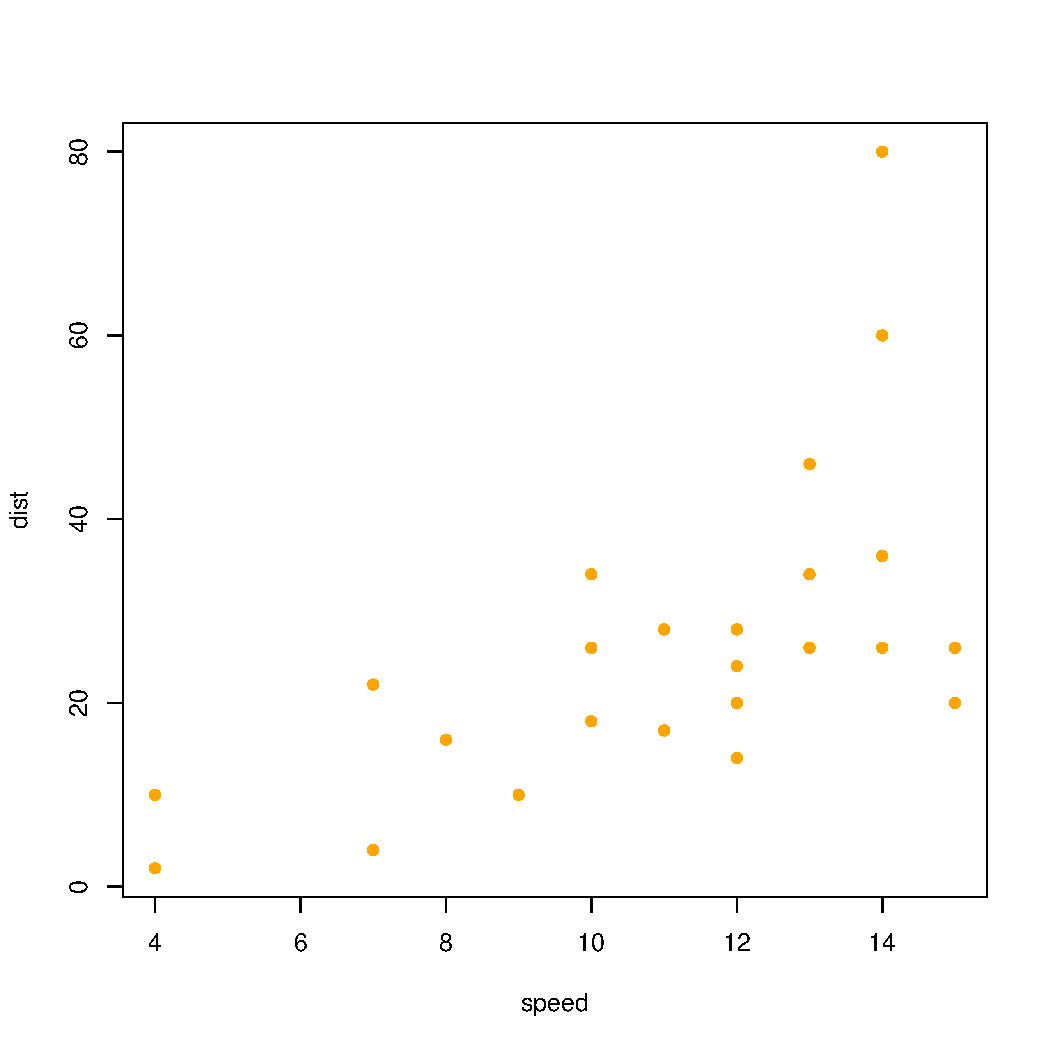
\includegraphics[height = 10cm, width = 10cm]{figure/report_3.pdf}
  \caption{The details of the plot of dist vs speed displayed by the graphics engine display list}
  	\label{figure_2.1}
\end{center}
\end{figure}

The example demonstrates how to access the graphics engine display list of a plot drawn by \texttt{plot}. The values of x and y, the labels of x-axis and y-axis been displayed.



\chapter{Standalone}
\section{The Perspective Plots \texttt{persp()}}
The Perspective Plots \texttt{persp()} is used to draw a surface over the x-y plane. Usually, it has three main argument, \textbf{x, y, z}. Where \textbf{x} and \textbf{y} are the locations of grid line which the value z been measured, \textbf{z} is a matrix which containing the values that been used to plot, or it is the matrix that been calculated by a specific function, such as 3-D mathematical functions. The following example shows how to draw a obligatory mathematical surface rotated sinc function on Perspective Plot. See figure \ref{figure_3.1}
\begin{Schunk}
\begin{Sinput}
> x = y = seq(-10, 10, length= 40)
> f = function(x, y) { r = sqrt(x^2+y^2); 10 * sin(r)/r }
> z = outer(x, y, f)
> z[is.na(z)] = 1
> trans = persp(x, y, z, theta=30, phi = 20, expand = 0.5,
+               col = 'White', border = 'orange')
\end{Sinput}
\end{Schunk}
\begin{figure}[h]
\begin{center}
  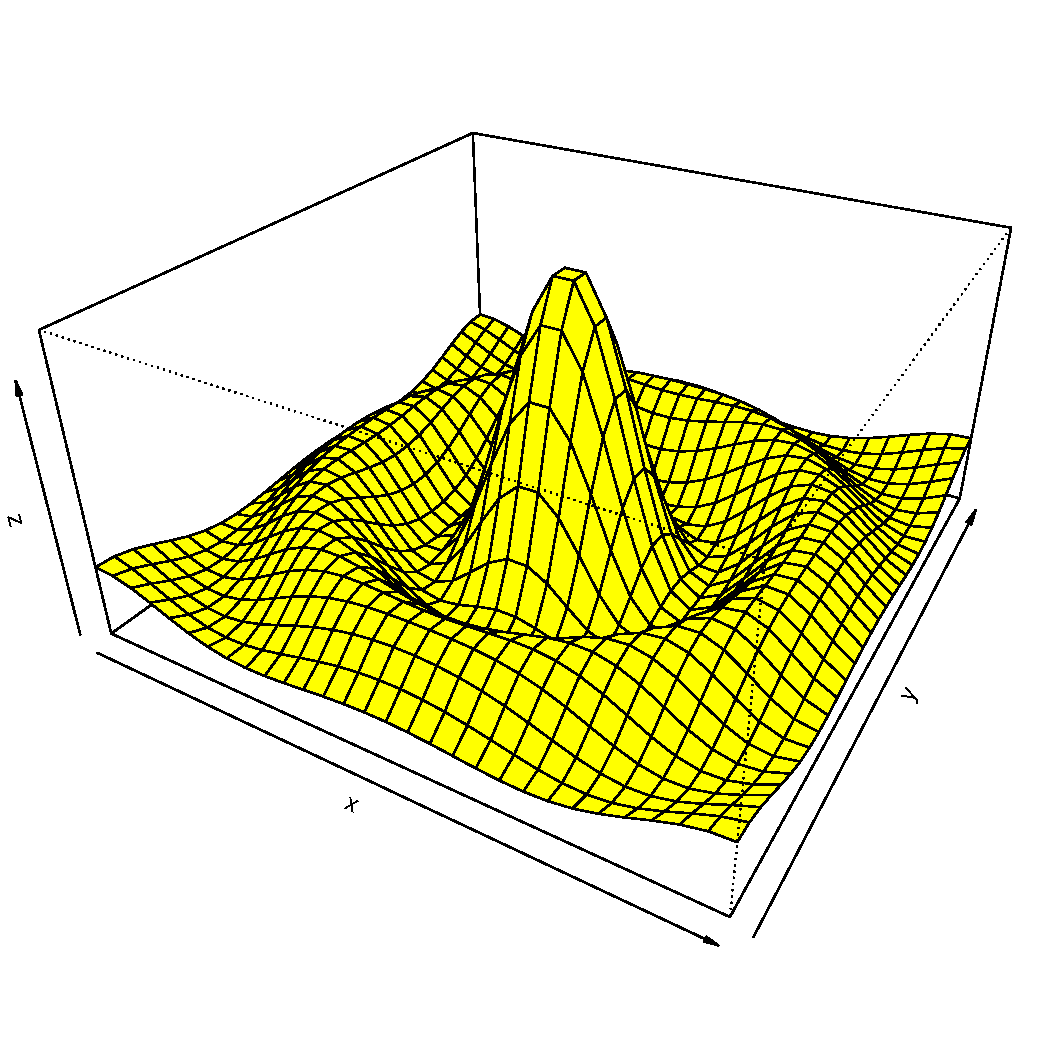
\includegraphics[height = 10cm, width = 10cm]{figure/standalone_1.pdf}
  \caption{An example of Perspective Plot been drawn by \texttt{persp()}}
  	\label{figure_3.1}
\end{center}
\end{figure}

It is clearly to see that the Perspective Plots is formed by a finite number of "polygon", each polygon has 4 Vertices. If we can access the values for each Vertices of the polygon, then we can reproduce this polygon. If we can access all the values of Vertices of all polygons, then we can reproduce the Perspective Plot. \\

Inorder to emulate this plot, we need to access some information from the graphics engine display list. However, the value of the vertices is not in the display list, therefore the plot cannot be reproduced directly. But we can access value of \textbf{x}, \textbf{y} and \textbf{z}, therefore we should re-do the calculation to get values of all vertices. The following codes show that the value of \textbf{x}, \textbf{y} and \textbf{z} which inputted by the user can been " caught " from the display list.
\begin{Schunk}
\begin{Sinput}
> reco = recordPlot()
> info = reco[[1]][[3]][[2]]
> ## print the values of x
> head(info[[2]])
\end{Sinput}
\begin{Soutput}
[1] -10.000000  -9.487179  -8.974359  -8.461538  -7.948718  -7.435897
\end{Soutput}
\begin{Sinput}
> ## print the values of y
> head(info[[3]])
\end{Sinput}
\begin{Soutput}
[1] -10.000000  -9.487179  -8.974359  -8.461538  -7.948718  -7.435897
\end{Soutput}
\begin{Sinput}
> ## print the values of z
> info[[4]][1:6, 1:2]
\end{Sinput}
\begin{Soutput}
            [,1]       [,2]
[1,]  0.70709805  0.6807616
[2,]  0.68076162  0.5602102
[3,]  0.56890062  0.3623630
[4,]  0.38799490  0.1144364
[5,]  0.16158290 -0.1521360
[6,] -0.08388565 -0.4067000
\end{Soutput}
\end{Schunk}
\subsection{The translation from 3-D points into 2-D points}
The values of \textbf{x}, \textbf{y} and \textbf{z} can been recored from the display list, which been explained by the previous section, the next task is to use this information to reproduce the vertics in 3-D.\\

As we know, the matrix, \textbf{z} is computed by a specific functions, given two inputs, \textbf{x} and \textbf{y}, or the expression of z can been written as: $z = f(x,y)$, it contains all the values for all combination of \empth{x} and \textbf{y} and the dimenstion of \textbf{z} is $ \textbf{length(x)} \times \textbf{length(y)}$.\\

One 3-dimenstions points contains a set values of $(x, y, z)$, but \textbf{z} is $\textbf{length(x)} \times \textbf{length(y)}$ matrix, \textbf{x} is a vector which has length of $\textbf{length(x)}$ and \textbf{y} is a vector which has length of $\textbf{length(y)}$. In order to produce the points, the D of \textbf{x}, \textbf{y} and \textbf{z} need to be matched and in a right order.\\

First step is the reduce the \textbf{Z} matrix into a one dimension vector which has length of $\textbf{length(x)} \times \textbf{length(y)}$. It can be reduced by either along x direction or y direction. In this paper, we reduced along the x direction. The second step is repeat the vector x and y until the same length of \textbf{z}. Since \textbf{z} is reduced along the x direction say $z_p$, hence we repeat x until the length of y say $x_p$, and we repeat each y by the length of \textbf{x}, say $y_p$. At last, the combination of $\x_p$, $y_p$, $z_p$ is the 3-D points which prepare for computing the vertices. \\
\begin{Schunk}
\begin{Sinput}
> xTmp = rep(x, length(y))
> yTmp = rep(y,each = length(x))
> zTmp = as.numeric(z)
> length(xTmp) == length(zTmp) & length(yTmp) == length(zTmp)
\end{Sinput}
\begin{Soutput}
[1] TRUE
\end{Soutput}
\end{Schunk}

The idea of transform the points into vertices is repeating the points in a right order. From previous section, we explained that the Perspective Plots is made by finite number of polygons. Each polygon has 4 vertices. The total number of polygons are required to be drawn is depend on the length of input \textbf{x} and the length of input \textbf{y}, that is, \textbf{total = (length(x) - 1) $\times$ (length(y) - 1)}. The polygons been drawn by connecting 4 points in a specific order. The algorithm of the drawing as follows: starting from bottom-left, first connect bottom-left to bottom-right, second connect from bottom-right to top-right, lastly, connect top-right to top-left. Every polygon is being drawn in this order. The surface of Perspective Plots is formed until all the polygons are been drawn. \\

Before drawing the surface, the transformation of 3-D vertices into 2-D vertices is required. This transformation required two main variables, the 3-D vertices and $4 \times 4$ viewing transformation matrix \textbf{P}. The 3-dimenstion vertices are computed, the matrix \textbf{P} can been recored from the \texttt{persp()} call. This transformation can be done easily on R by using the \texttt{trans3d()} function.

\begin{Schunk}
\begin{Sinput}
> points3d = trans3d(xTmp, yTmp, zTmp, trans)
> head(points3d$x)
\end{Sinput}
\begin{Soutput}
[1] -0.3929051 -0.3827005 -0.3720915 -0.3611435 -0.3499392 -0.3385634
\end{Soutput}
\begin{Sinput}
> head(points3d$y)
\end{Sinput}
\begin{Soutput}
[1] -0.1060481 -0.1099038 -0.1156894 -0.1230654 -0.1315269 -0.1404974
\end{Soutput}
\end{Schunk}

Because of we are drawing a 3-D surface in a 2-D plane, some polygons that stay 'behind' cannot been seen, it is necessary to draw the polygons in a right order. The order defined by using the \textbf{x} and \textbf{y} coordinate of the 3-D vertices (but ignore the \textbf{z} coordinate) combining another column \textbf{1}, then do the matrix multiplication with the viewing transformation \textbf{P}. The fourth column from this multiplication is the drawing order of the polygons.
\begin{Schunk}
\begin{Sinput}
> orderTemp = cbind(xTmp, yTmp, 0, 1) %*% trans 
> zdepth = orderTemp[, 4]
> ## the zdepth of a set of 4 points of each polygon
> a = order(zdepth, decreasing = TRUE)
> head(a)
\end{Sinput}
\begin{Soutput}
[1] 1561 1562 1521 1563 1522 1564
\end{Soutput}
\end{Schunk}

Figure \ref{figure_3.2} shows how does this paper approximate to the solution. The top-left figure is drawn by plotting the transformed 2-dimenstion points, the shape of the Perspective Plots been presented. The top-right figure is drawn by connecting the points line-by-line, the shape become more obvious. The bottom-left figure is drawn by using the \texttt{grid.polygon()}. By default, the origin order of the polygons is drawn along x-axis, then along y-axis. Clearly this is not the correct order. Finally, the bottom-right figure shows the true Perspective Plots by fixing the order. 
\newpage
\begin{figure}[h]
\begin{center}
  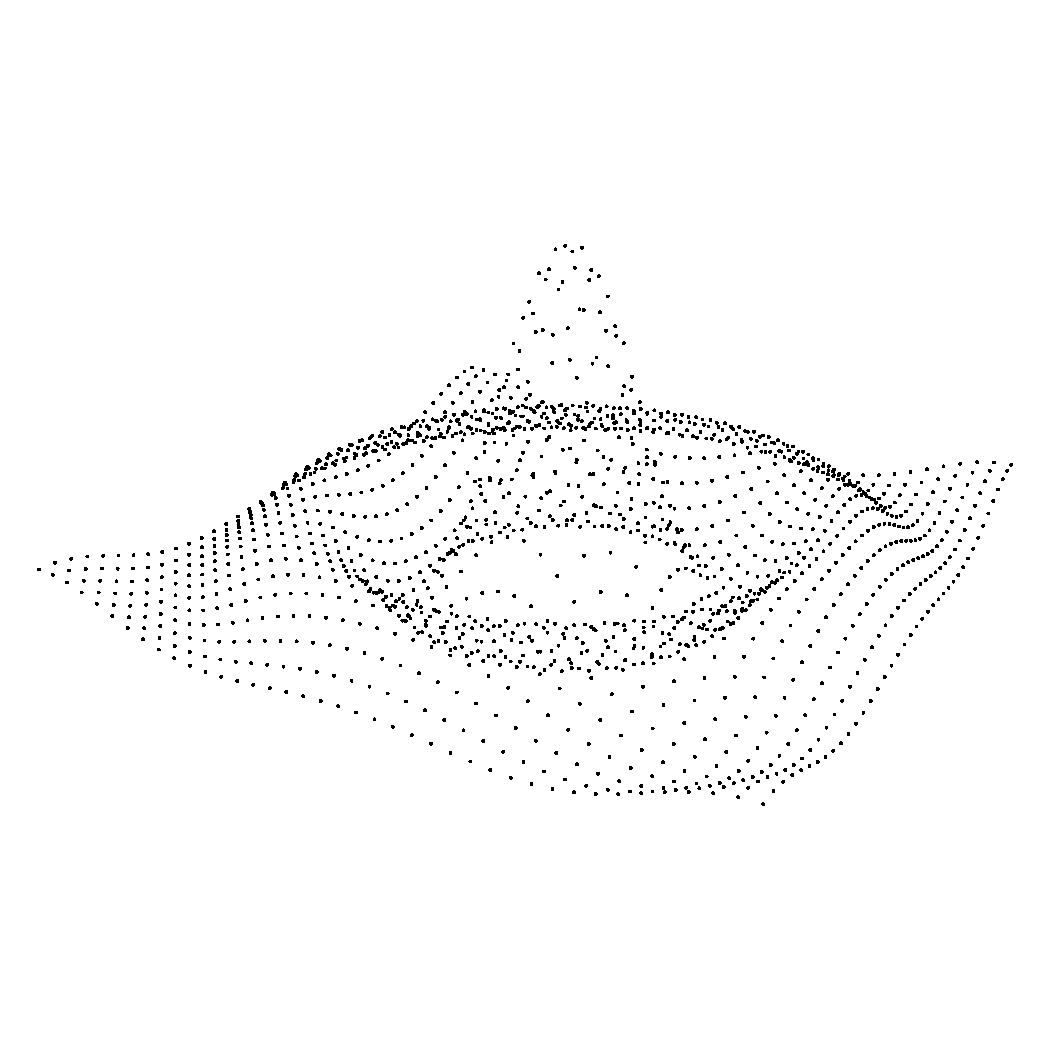
\includegraphics[height = 7.5cm, width = 7.5cm]{figure/standalone_p_1.pdf}
  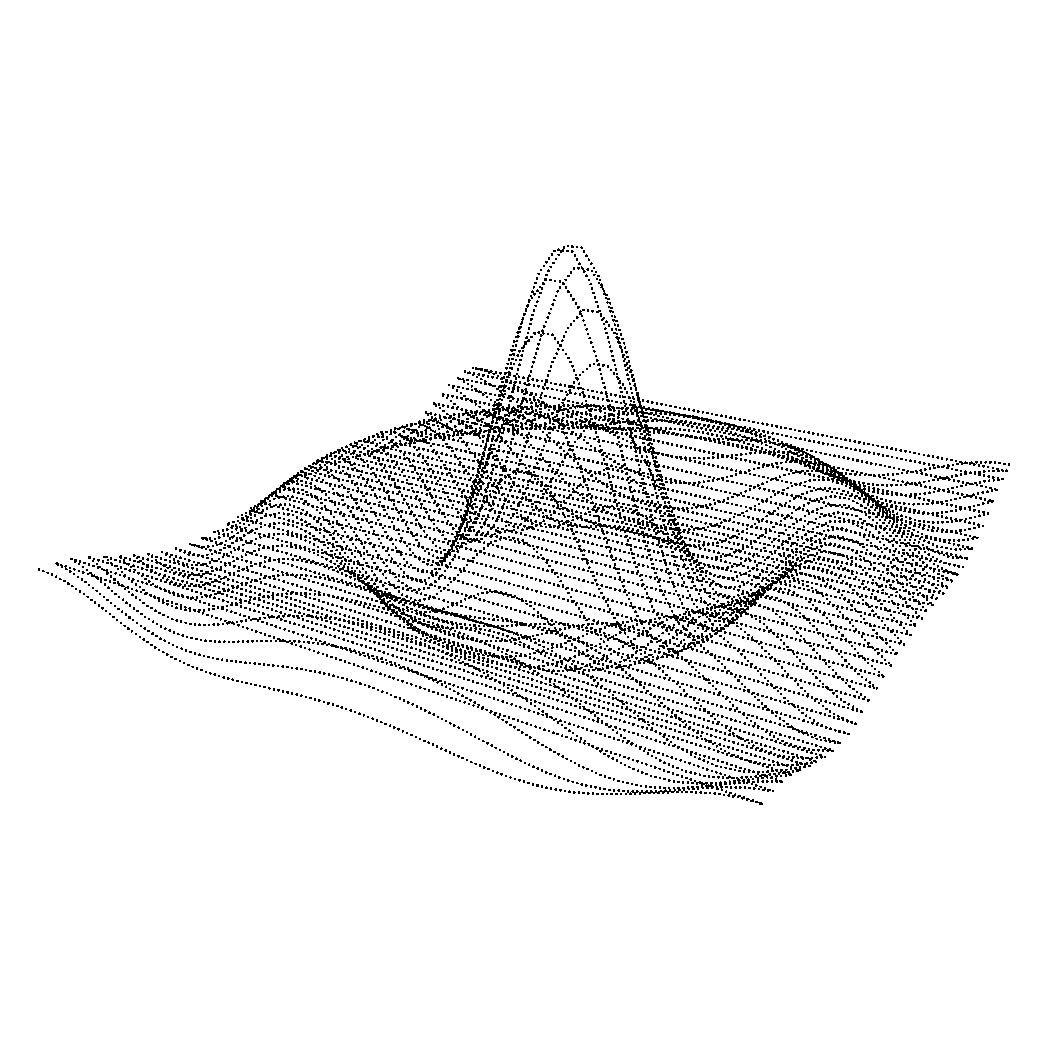
\includegraphics[height = 7.5cm, width = 7.5cm]{figure/standalone_p_2.pdf}
  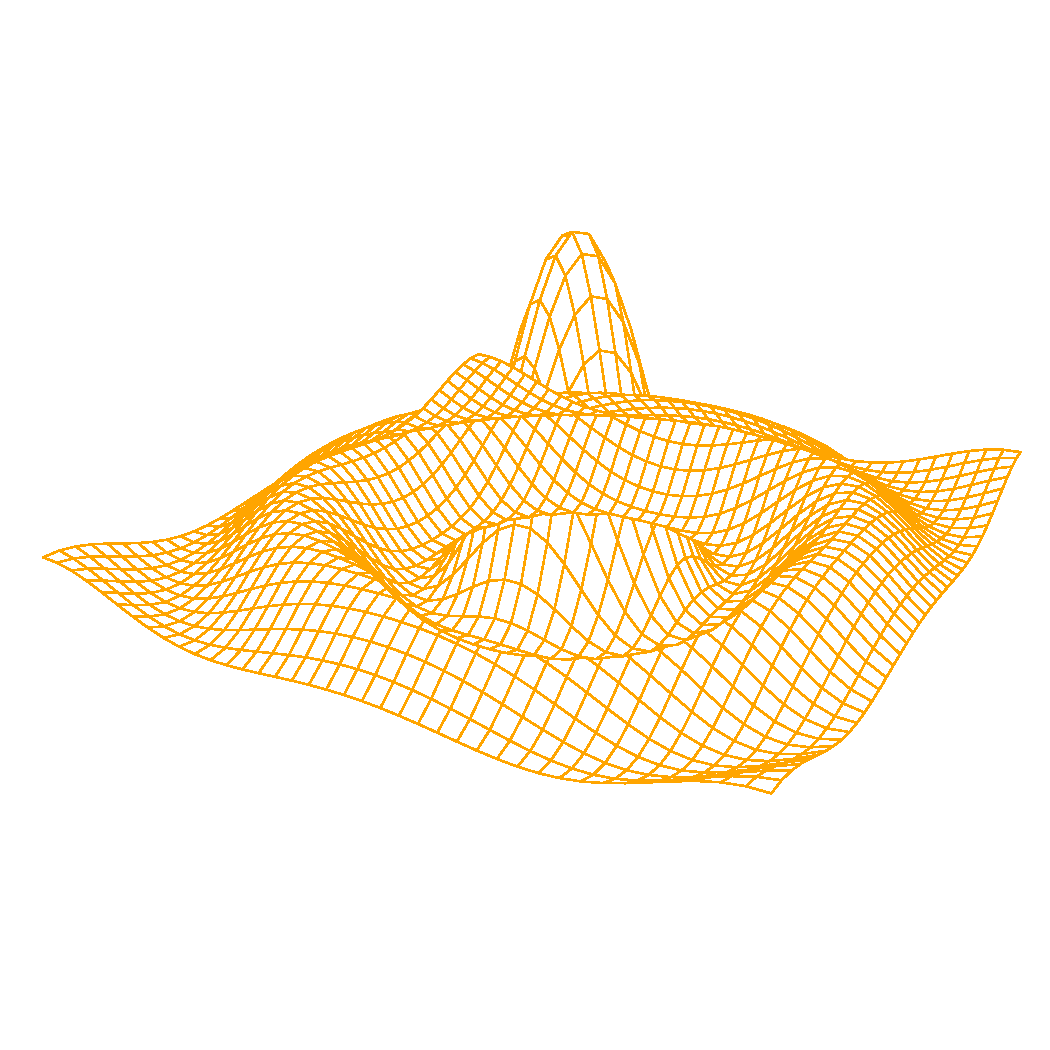
\includegraphics[height = 7.5cm, width = 7.5cm]{figure/standalone_p_3.pdf}
  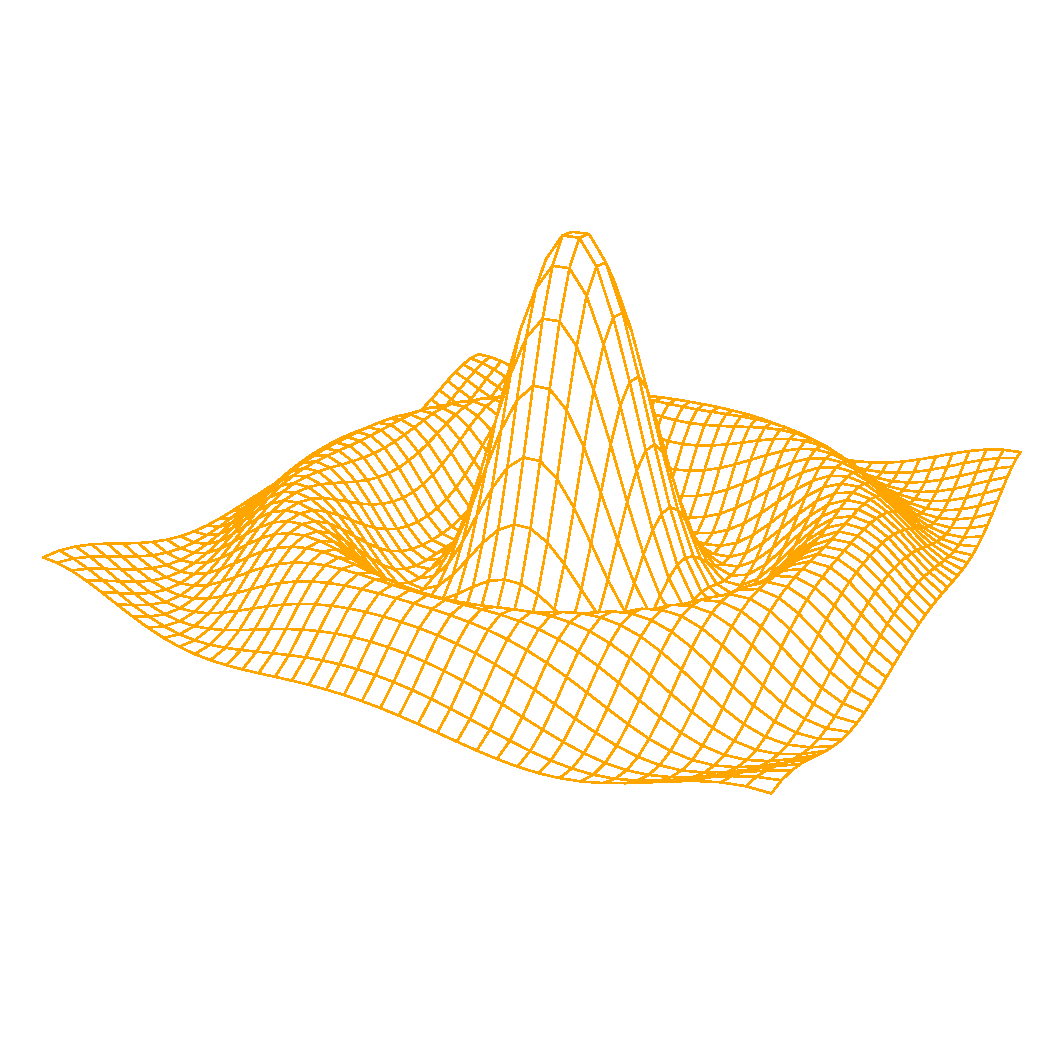
\includegraphics[height = 7.5cm, width = 7.5cm]{figure/standalone_p_4.pdf}
  \caption{The top-left figure is only plotting the transformed 2-dimenstion points. The top-right figure is being drawn by connecting the points line-by-line. The top-right figure is drawn unorderly by using the \testtt{grid.polygon}. Finally, the bottom-left figure is drawn in a correct order.}
  	\label{figure_3.2}
\end{center}
\end{figure}

\subsection{Lighting}
The other main benefit supported by \texttt{persp()} is the shading. It shades the surface by assuming the surface is being illuminated from a given direction. (light source) \\

In \texttt{persp()}, the main parameters that the user needs to specify for producing a shaded perspective plot is: \textit{ltheta}, \textit{lphi} and \textit{shade}.\\

\textit{ltheta} and \textit{lphi} are used for setting up the direction of the light source. In particular, \textit{ltheta} specifies the angle in the z direction, \textit{lphi} specifies the angle in the x direction. \\

\textit{shade} is the parameter that specifies the shade at each facets of the surface, and the shades will be computed as follows:
\begin{equation}
\big(\frac{1 + d}{2}\big)^{shade}
\end{equation}
Where \textit{d} is the dot product of the unit vector normal to each facet (\textit{u}) and the unit vector of the direction of the light(\textit{v}). \\

The color of each facet will be calculated by the color that is recored from the graphics engine display list multiplied by the \textbf{shade}. Finally, the surface is drawn by filling the colors for every facet.\\

If the normal vector is perpendicular to the direction of the light source, then $d = 0$ and the term $\big(\frac{1 + d}{2}\big)^{shade}$ will be close to 0, therefore the corrosponding facets will become darker. The brightness and darkness will depend on the value of the \textbf{shade}. If shade close to 0, the term $\big(\frac{1 + d}{2}\big)^{shade}$ will be close to 1. Therefore, it will look like non-shading plot. Similarly, if the shade gets larger, the term close to 0 and the plot gets darker.

\begin{Schunk}
\begin{Sinput}
> trans = persp(x, y, z, theta=30, phi = 20, expand = 0.5,
+  col = 'white', border = 'orange')
> trans = persp(x, y, z, theta=30, phi = 20, expand = 0.5,
+  col = 'white', border = 'orange', 
+  shade = 0.8, ltheta = 30, lphi = 20)
\end{Sinput}
\end{Schunk}


\begin{figure}[h]
\begin{center}
  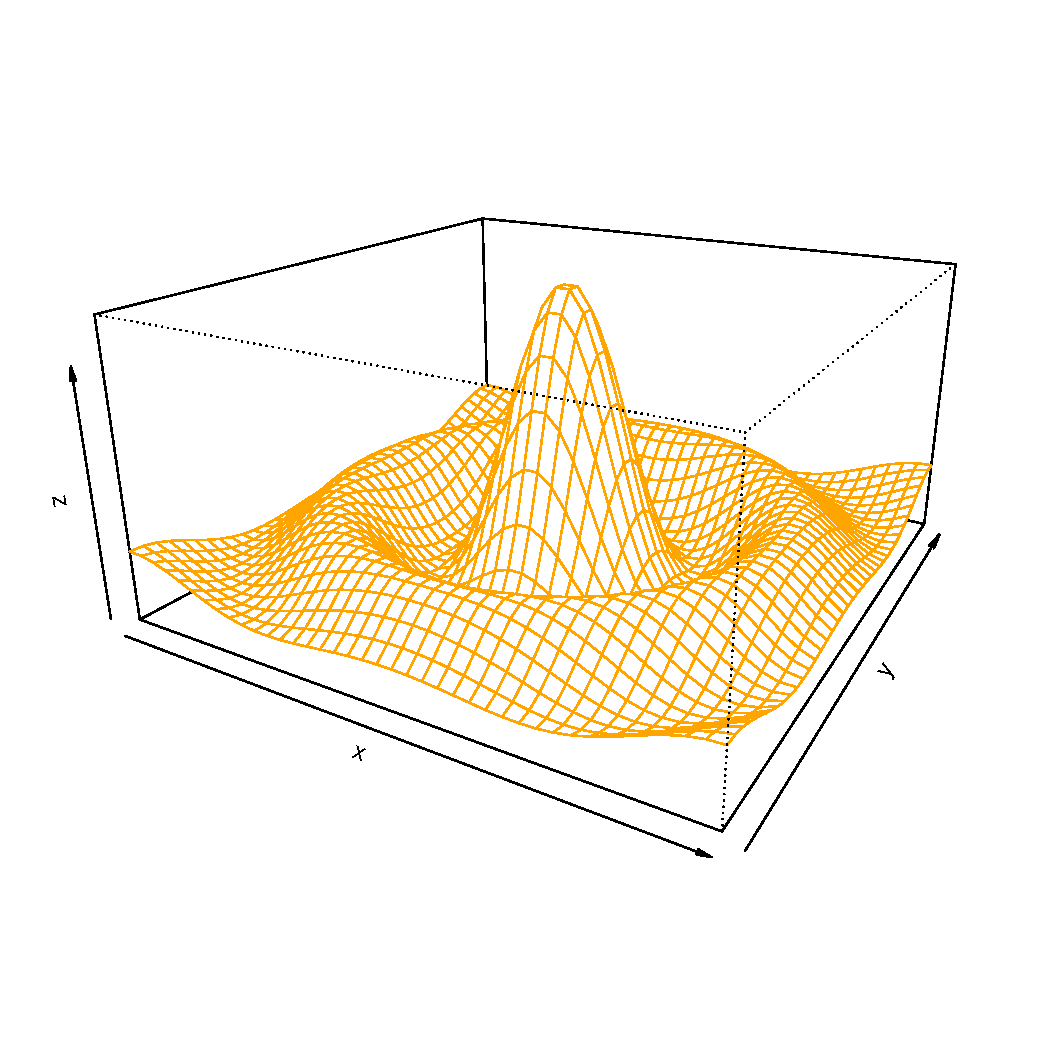
\includegraphics[height = 7.5cm, width = 7.5cm]{figure/Lighting_1.pdf}
  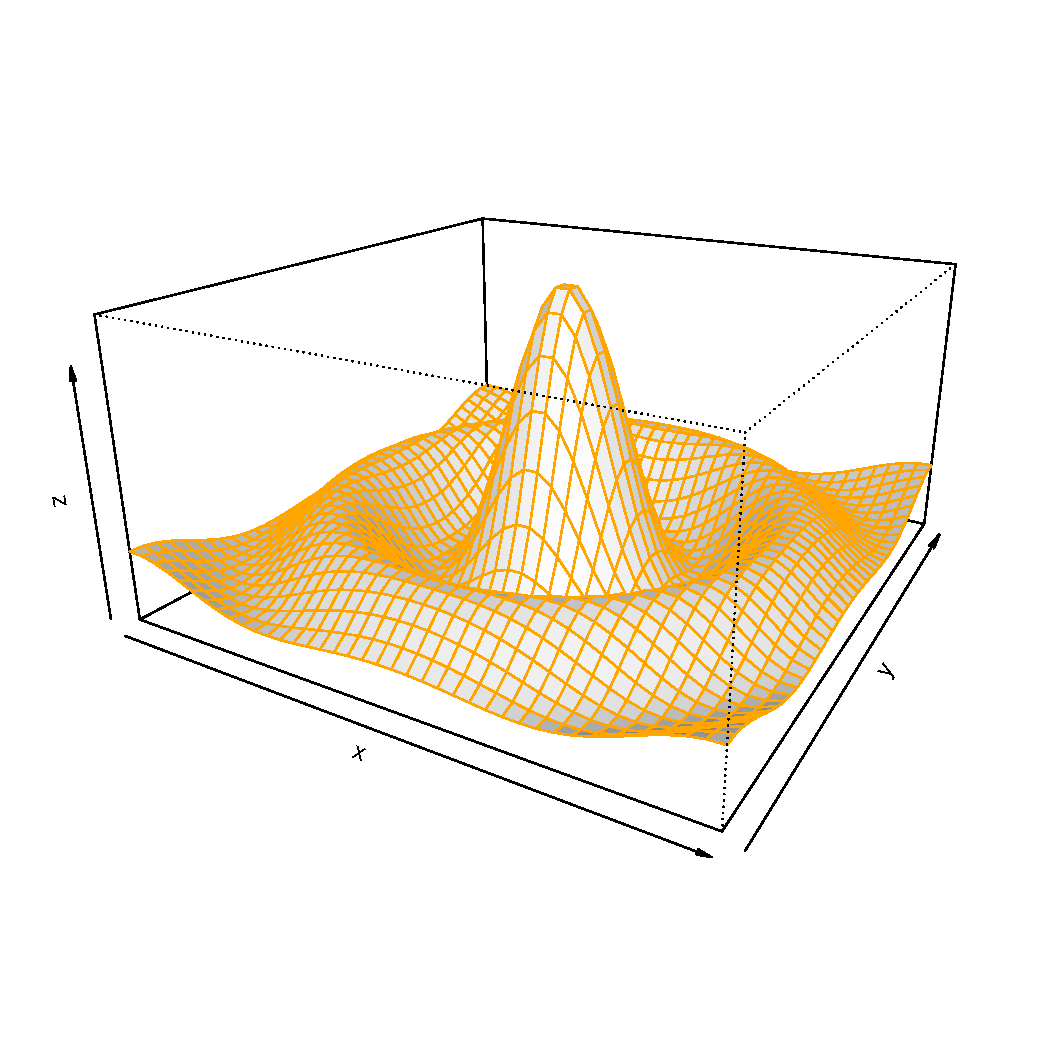
\includegraphics[height = 7.5cm, width = 7.5cm]{figure/Lighting_2.pdf}
  \caption{Adding a light source to the perspective plot from the same angel of view. The left plot is origin plot without shadding, where the right plot is been shaded.}
  	\label{figure_3.3}
\end{center}
\end{figure}

\subsection{Difference beween \texttt{C} and \texttt{R}}
Many functions in \texttt{R} call \texttt{C} code to do a lot of the work.  This is the case for \texttt{persp()} and \texttt{filled.contour()}. Although the structure of \texttt{C} code is quite similar to \texttt{R} code in some special cases, there are some \texttt{C} code structures which behave completely different to \texttt{R}, therefore translating \texttt{C} code to \texttt{R} code is not just "copy-and-paste".\\

\subsubsection{Pointers}
One main data structure in \texttt{C} is the pointer, which is a type of reference that records the address/location of a global object or a local variable in a function. Pointers can be manipulated by using assignment or pointer arithmetic.
\begin{lstlisting}
static int LimitCheck(double *lim, double *c, double *s)
{
    if (!R_FINITE(lim[0]) || !R_FINITE(lim[1]) || lim[0] >= lim[1])
    return 0;
    *s = 0.5 * fabs(lim[1] - lim[0]);
    *c = 0.5 * (lim[1] + lim[0]);
    return 1;
}
\end{lstlisting}

The top piece of code is used for checking the Limit for the \texttt{persp()} function. It also multiplying the variable \textttt{c} and \texttt{s} for further calculation. In this case, the \texttt{c*} and \texttt{s*} are the pointer which will point to the machine memory of \texttt{s} and \texttt{c} and modify them.\\

However, this process cannot be reproduced on \texttt{R} because \texttt{R} does not have the pointer data structure. One possible solution will be rather than doing the Limit checking and multiply \texttt{s} and \texttt{c}, do the limit checking and return/assign the \texttt{s} and \texttt{c} as \texttt{xs} ad \texttt{ys} for further calculation.
\begin{lstlisting}
LimitCheck = function ( lim ) {
    s = 0.5 * abs(lim[2] - lim[1])
    c = 0.5 * (lim[2] + lim[1])
    c(s, c)
}
xs = LimitCheck(xr)[1]
xc = LimitCheck(xr)[2]
...
\end{lstlisting}
\subsubsection{Array}
The other main difference is that \texttt{C} use array data format rather than matrix data format in \texttt{R}. However, the indexing of elements in matrix is identical to the indexing of elements in array. 
\begin{lstlisting}
FindPolygonVertices(c[k - 1], c[k],
        x[i - 1], x[i],
        y[j - 1], y[j],
        z[i - 1 + (j - 1) * nx],
        z[i + (j - 1) * nx],
        z[i - 1 + j * nx],
        z[i + j * nx],
        px, py, pz, &npt);
	    

out = lFindPolygonVertices(sc[k], sc[k + 1],
        x[i], x[i + 1],
        y[j], y[j + 1],
        z[i, j],
        z[i + 1, j],
        z[i, j + 1],
        z[i + 1, j + 1],
        px, py, pz, npt)
\end{lstlisting}

\textcolor{red}{
To get the same elements in the matrix as the elements in the array, one solution will be that
changing the matrix data format into vector data format. However, \texttt{R} is farmillar with matrix data structure. Hence it is easiler and more understandable by \texttt{R} user and programmer. The \texttt{z[i - 1 + (j - 1) * nx]} in \textt{FindPolygonVertices()} is selecting the $i^{th}$ element from the $j^{th}$ column. On the other word, it selected the $i^{th}$ row and $j^{th}$ element from a matrix, which the following \texttt{R} code provied the same result That is, \texttt{z[i, j]} in \texttt{R} will provide the same result as \texttt{C}
}\\

% get the "same" elements in the matrix as the elements in the array, one solution will be that changing the matrix data format into vector data format, so that the elements will be stay the same location for both array, and matrix data format.\\

The top piece of codes is both calling the \texttt{FindPolygonVertices()} function by feeding parameter into it. However, the \texttt{z} is array in the first call as it written on \texttt{C} but the second is matrix as it written on \texttt{R}. the - 1 on the \texttt{R} code because \texttt{C} starting at 0 index but \texttt{R} starting at 1.\\

\subsection{Box and other features}
One feather that \texttt{persp()} supported is whether draw a container (box) around the surface. (See figure \ref{figure_3.4}). Therefore, it is necessary to find out whether the edge of the box in front of the surface or behind the surface. \\ 
\textcolor{red}{Maybe rewrite this paragraph?} \\

The solution will be that translates the \texttt{C} code to \texttt{R} code directly. The reason for doing this directly translation is that R is sensitive on drawing the dot lines. More specifically, it may cause difference if we connect two points with a dotted line in different direction. Due to the purpose of this paper, the plot should be drawn as identical as possible. Therefore, the direct translation is required.\\


\begin{figure}[h]
\begin{center}
  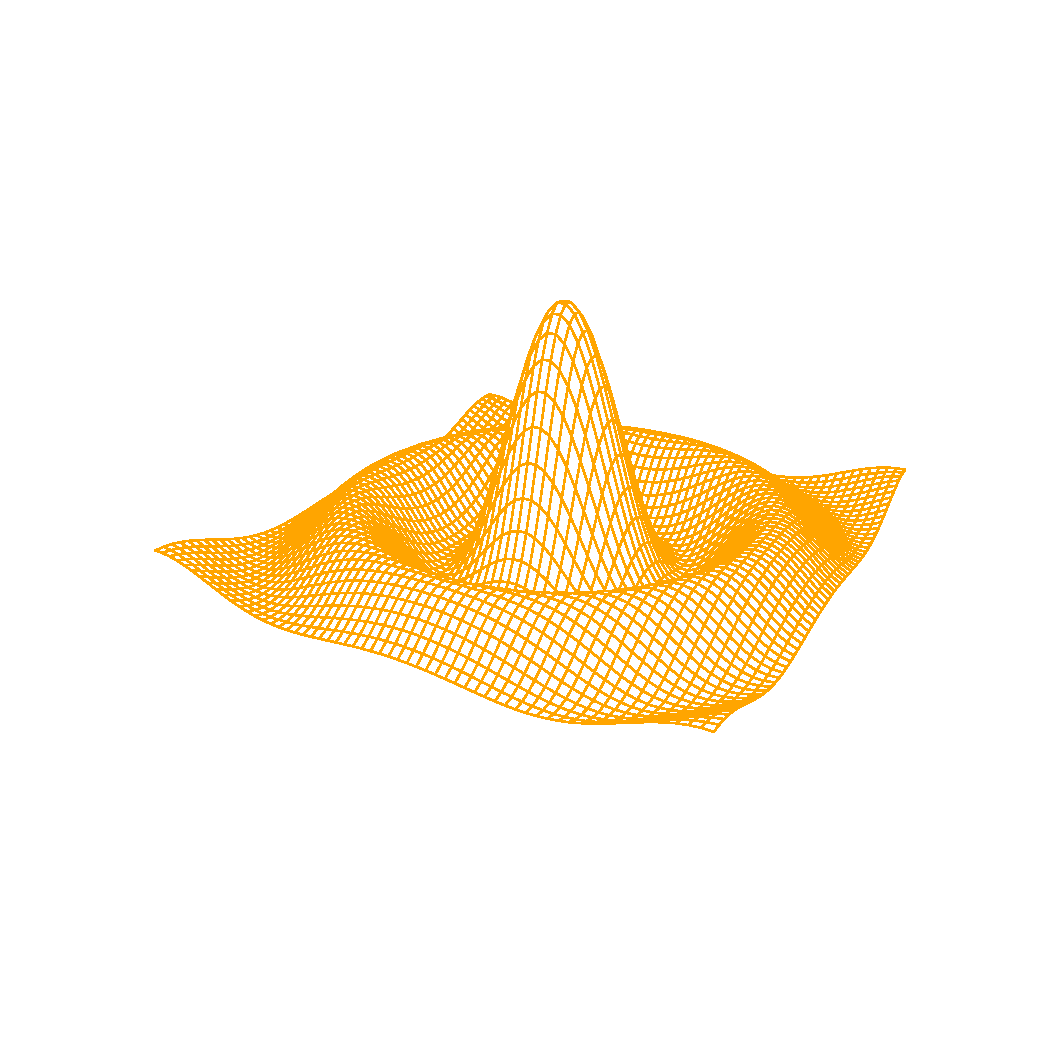
\includegraphics[height = 7.5cm, width = 7.5cm]{figure/box_example_1.pdf}
  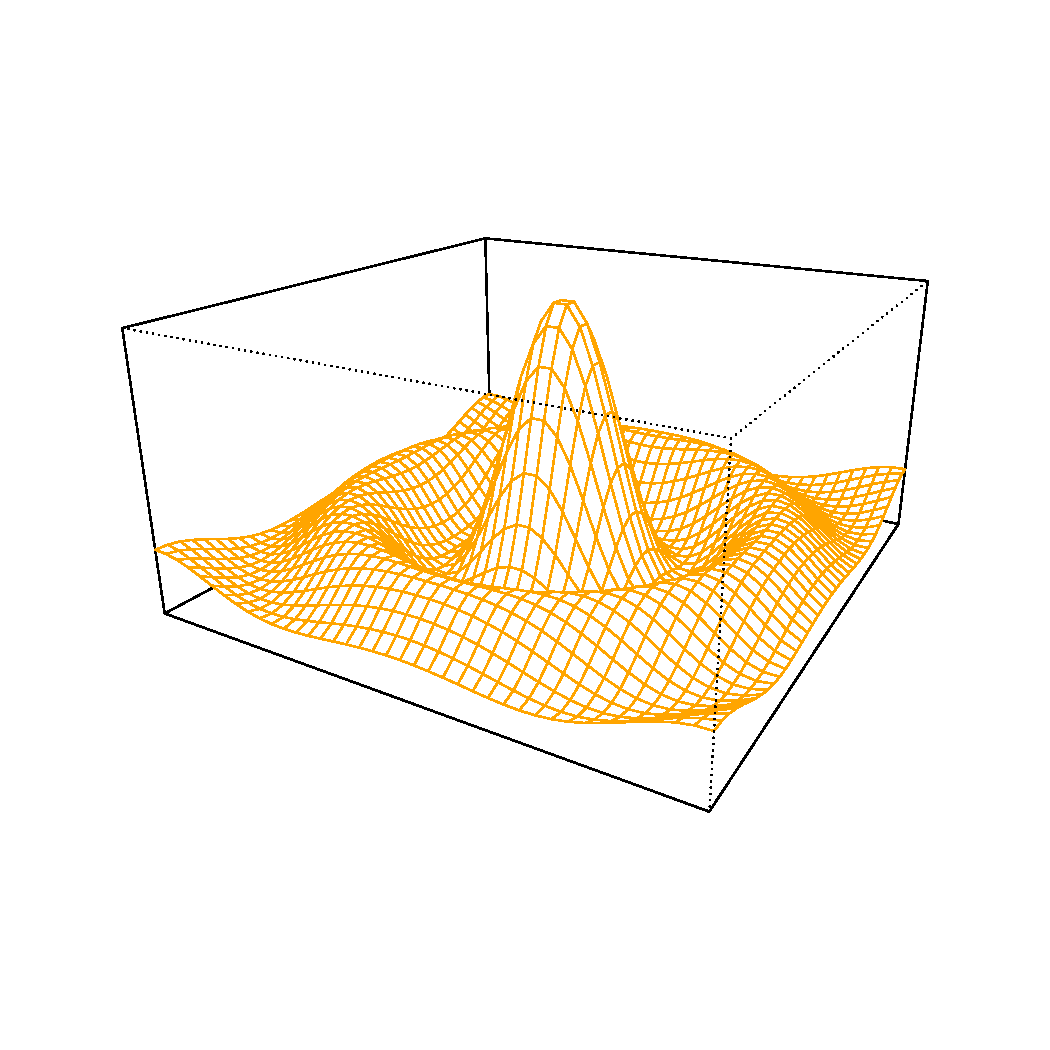
\includegraphics[height = 7.5cm, width = 7.5cm]{figure/box_example_2.pdf}
  \caption{The surace been drawn by ignore the box in the left plot, right plot drawn the surface as well as box}
  	\label{figure_3.4}
\end{center}
\end{figure}

Other feather that \texttt{persp} supported is the detail of the axis.(See figure \ref{figure_3.5}) More specifily, the axis has three type, no axes, simple axes which only contain the label of axes, or showing the scale of each axes. These feathers are required to be reproduced by \texttt{grid}, The solution to this problem by translating the \texttt{C} code to \texttt{R} code directly.



\begin{figure}[h]
\begin{center}
  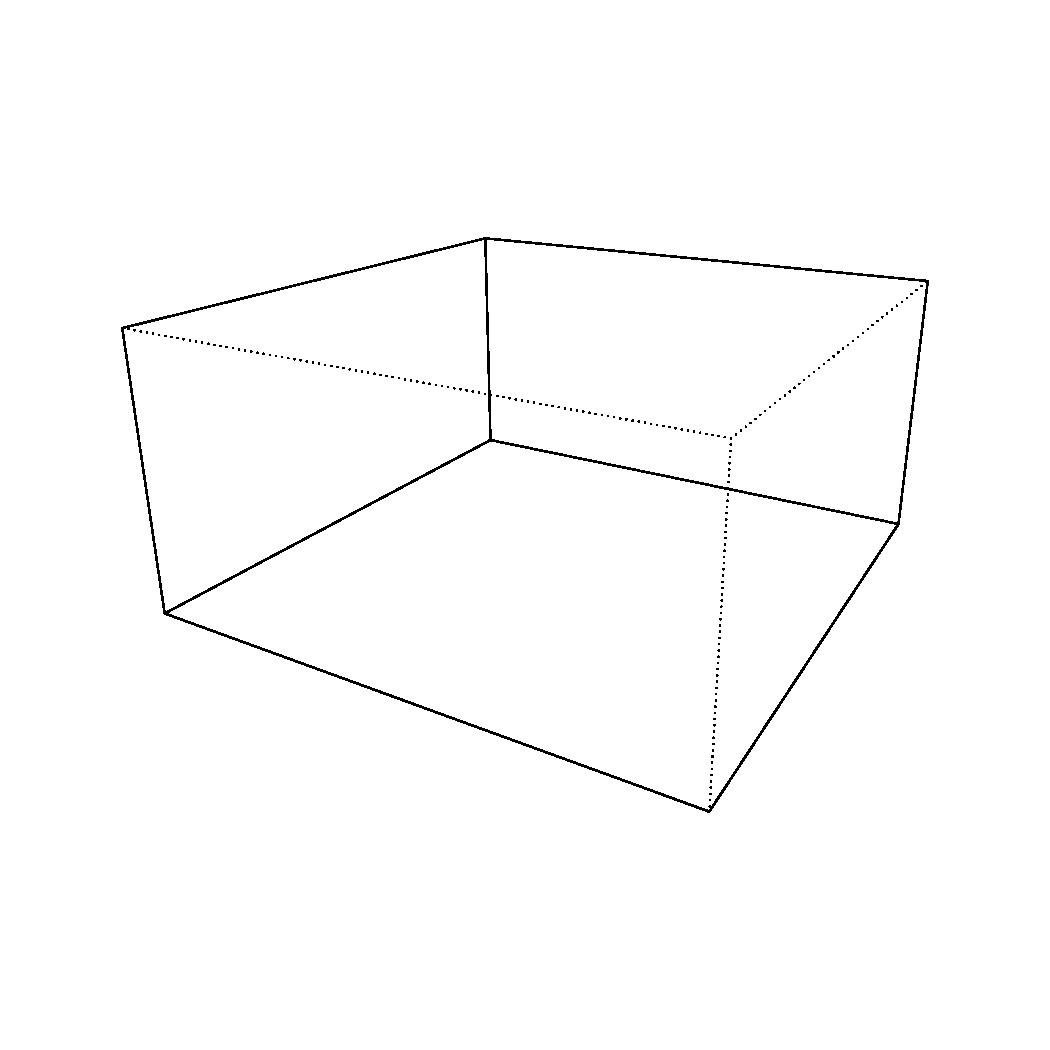
\includegraphics[height = 5cm, width = 5cm]{figure/axis_example_1.pdf}
  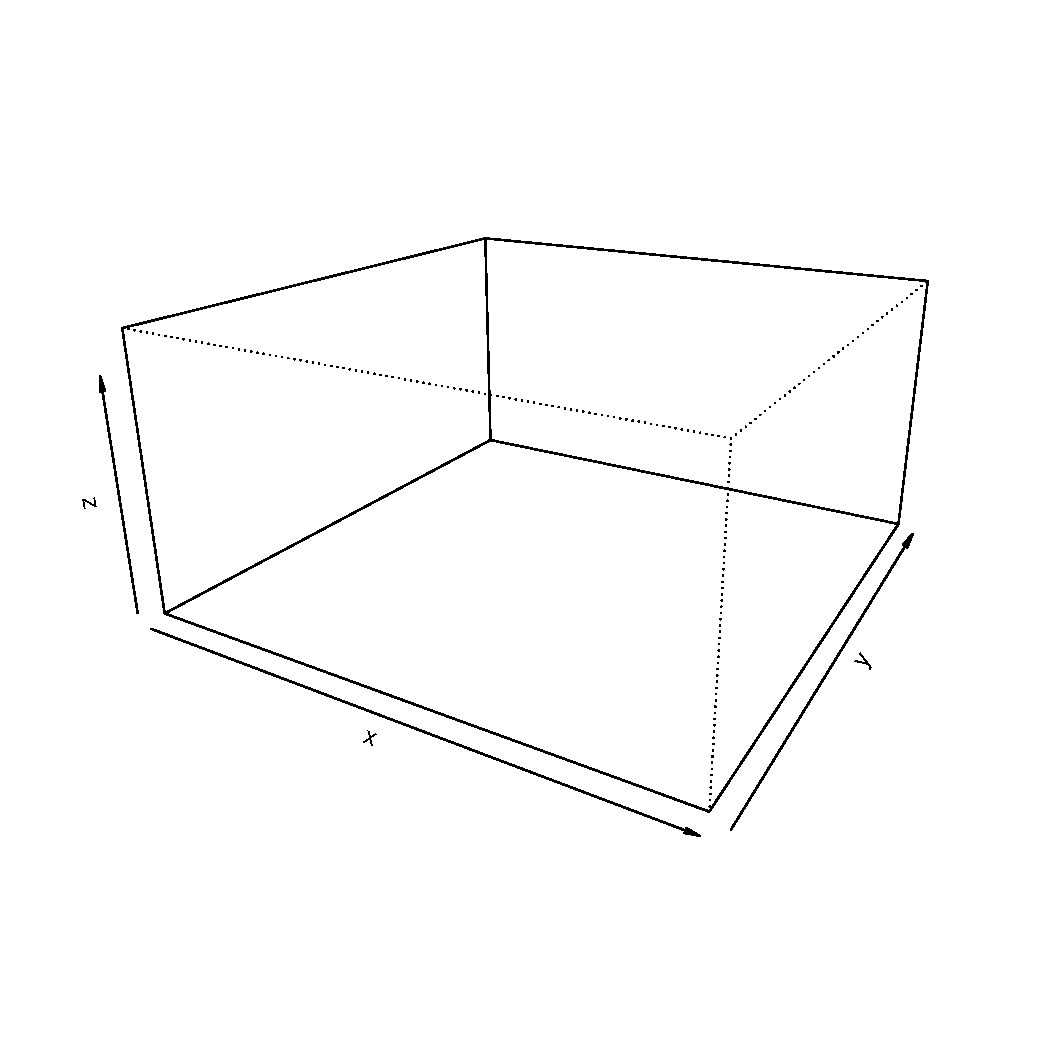
\includegraphics[height = 5cm, width = 5cm]{figure/axis_example_2.pdf}
  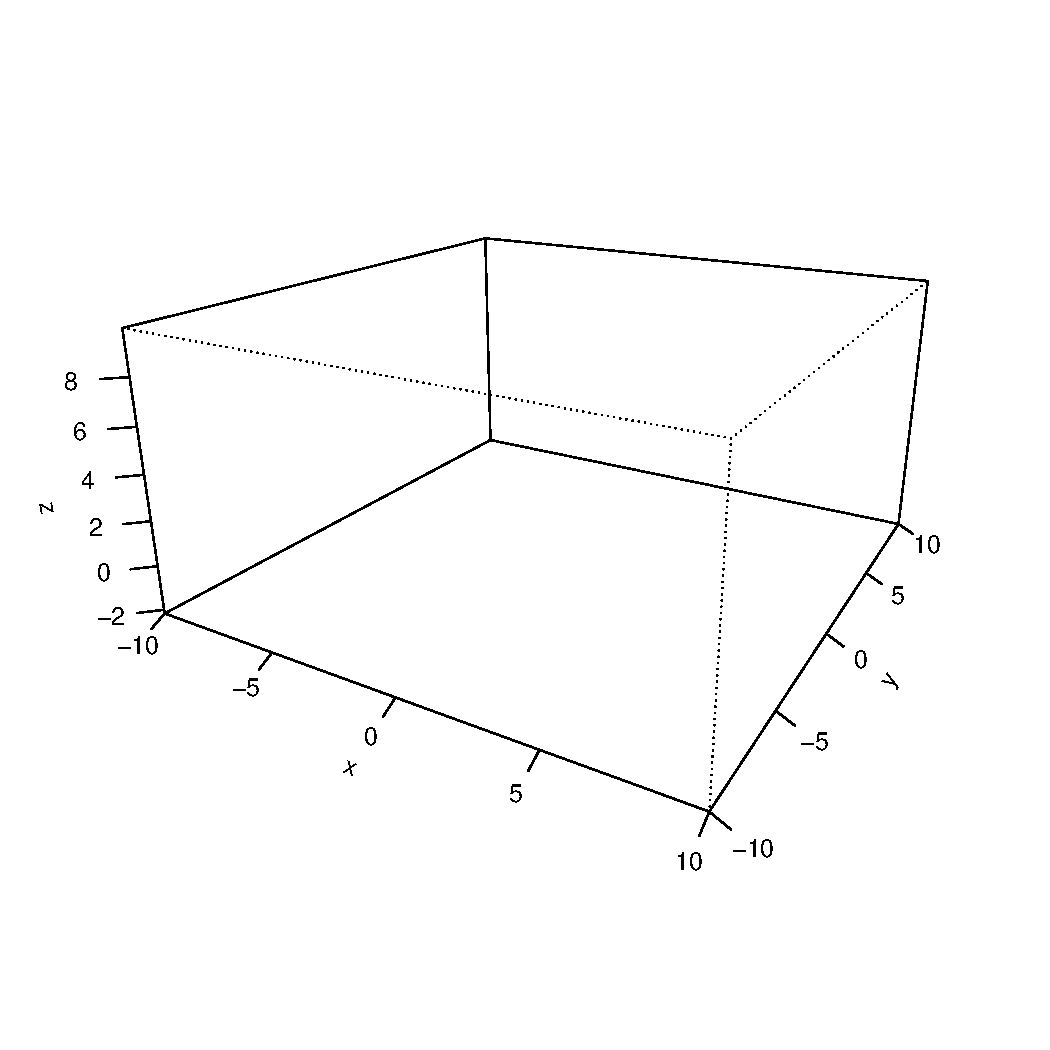
\includegraphics[height = 5cm, width = 5cm]{figure/axis_example_3.pdf}
  \caption{The Perspective surfaces are been ignored in this example, the left plot shows no axis been drawn, the simple axes been drawn in the middle plot and the right plot shows more detail for each axis.}
  	\label{figure_3.5}
\end{center}
\end{figure}

\section{The Filled Contour Plot}
\subsection{Direct translation from \texttt{C} to \texttt{R}}
The other tasks of this paper is to emulate the Level (Contour) Plots (\texttt{filled.contour}) from \texttt{graphics} to \texttt{grid}. As previous section, the first step to emulate \texttt{filled.contour} is to access the information from the graphics engine display list. (See figure \ref{figure_3.6})
\begin{Schunk}
\begin{Sinput}
> x = 10*1:nrow(volcano)
> y = 10*1:ncol(volcano)
> filled.contour(x, y, volcano, color = terrain.colors,
+     plot.title = title(main = "The Topography of Maunga Whau",
+     xlab = "Meters North", ylab = "Meters West"),
+     plot.axes = { axis(1, seq(100, 800, by = 100))
+                   axis(2, seq(100, 600, by = 100)) },
+     key.title = title(main = "Height\n(meters)"),
+     key.axes = axis(4, seq(90, 190, by = 10)))
> xx = recordPlot()
> info = xx[[1]][[12]][[2]]
> head(info[[2]])  ## print the values of x
\end{Sinput}
\begin{Soutput}
[1] 10 20 30 40 50 60
\end{Soutput}
\begin{Sinput}
> head(info[[3]])  ## print the values of y
\end{Sinput}
\begin{Soutput}
[1] 10 20 30 40 50 60
\end{Soutput}
\begin{Sinput}
> dim(info[[4]])  ## print the dimension of z
\end{Sinput}
\begin{Soutput}
[1] 87 61
\end{Soutput}
\begin{Sinput}
> length(info[[5]])  ## print the length of s
\end{Sinput}
\begin{Soutput}
[1] 22
\end{Soutput}
\end{Schunk}
\begin{figure}[h]
\begin{center}
  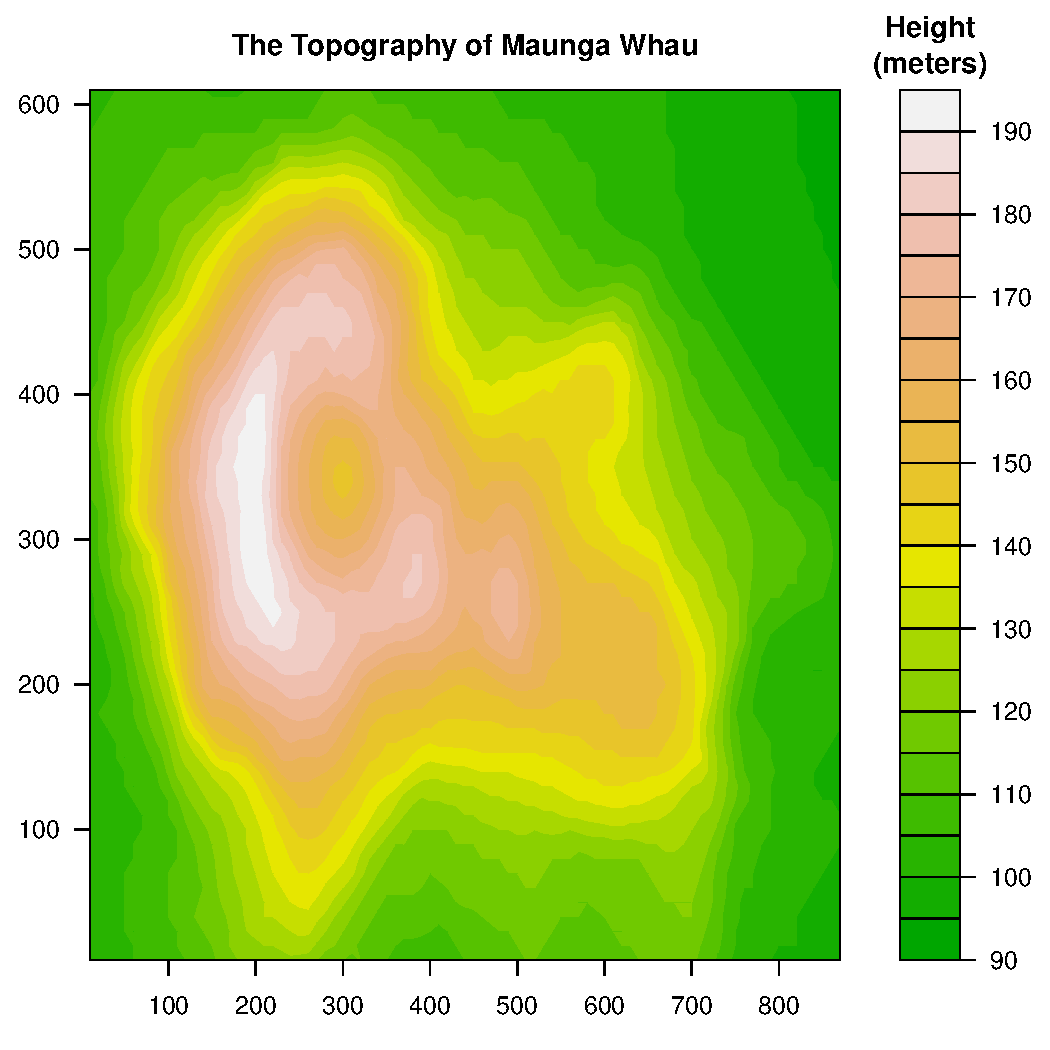
\includegraphics[height = 10cm, width = 12cm]{figure/filled_example_1.pdf}
  \caption{The topography of the Maunga Whau been drawn by using the \texttt{filled.contour}}
  	\label{figure_3.6}
\end{center}
\end{figure}
The example shows the plot of topography of Maunga Whau and also the information from the \texttt{filled.contour} call in the graphics engine display list. Same problem as \texttt{persp()}, there is no way to reproduce this plot directly by only using the coordinates of x, y and z.\\

There is an algorithm to create this contour plot in the \texttt{graphics} package written by \texttt{C}. The first step of the solution will be translated the \texttt{C} code directly to maximize the accuracy.\\

\begin{lstlisting}
static void
FindPolygonVertices(..., double *x, double *y, double *z, int *npt, ...)
{
  *npt = 0;
  FindCutPoints(low, high, x1,  y1,  z11, x2,  y1,  z21, x, y, z, npt);
  FindCutPoints(low, high, y1,  x2,  z21, y2,  x2,  z22, y, x, z, npt);
  FindCutPoints(low, high, x2,  y2,  z22, x1,  y2,  z12, x, y, z, npt);
  FindCutPoints(low, high, y2,  x1,  z12, y1,  x1,  z11, y, x, z, npt);
}
\end{lstlisting}
This piece of \texttt{C} code is the algorithm used for calculate the coordinates of the vertex of each polygon in the level contour plot. The parameters $*x$, $*y$, $*z$ are the array pointers which have length of 8 individually, $*npc$ is also a pointer has length of 1. If the \texttt{FindCutPoints} is called, the elements in the arrays of $x$, $y$, $z$ will be modified. In general, we feed the location of memory of $x$, $y$, $z$ and $npt$ to \texttt{FindPolygonVertices()} and modify the values of $x$, $y$, $z$ and $npt$ within the \texttt{FindCutPoints}.\\

For example, the first call of \texttt{FindCutPoints()} modifies the elements in the pointer arrays of $x$, $y$, $z$. The location of elements in arrays been modified will depend on the parameter $*npt$. More specifically, the $*x$ as a function of $x_1$ and $x_2$, $y$ as a function of $y_1$ and so on. The second \texttt{FindCutPoints()} is slightly different, $x$ will depend on a function of $x_2$, $y$ as a function of $y_1$ and $y_2$. In the third \texttt{FindCutPoints()} call, $x$ will depend on a function of $x_2$ and $x_1$, $y$ will depend on a function of $y_2$. Finally, $x$ will depend on a function of $x_1$, $y$ depend on the function of $y_2$ and $y_1$. \\

There is no pointer data structure in \texttt{R} hence we cannot produce the same action as \texttt{C}. One approximation to this action will be as follows:
\begin{lstlisting}
lFindPolygonVertices = function(...)
{
    out = list(); npt = 0
    out1 = lFindCutPoints(...)
    x = y = z = numeric(8); npt = out1$npt
    ...
    out$x = out1$x + out2$y + out3$x + out4$y
    out$y = out1$y + out2$x + out3$y + out4$x
    out$npt = out4$npt
    out
}
\end{lstlisting}
Instead of mortify $x$, $y$, $z$ and $npt$ inside \texttt{FindCutPoints()}, record the values for $x$, $y$, $z$ and $npt$ outside the \texttt{lFindCutPoints()} call in \texttt{R} every time. At last, we combined every $x$ and $y$ together as the previous \texttt{C} code behave. 


\subsection{Vectorization}
In \texttt{C}, the total iteration in the loops is equal to
\begin{equation}
Total = nx * ny * ns
\end{equation}
Where:\\
$nx = length(x) - 1$,\\
$ny = length(y) - 1$,\\
$ns = length(levels) - 1$\\
It requires huge iteration. For example, In Figure \ref{figure8}, the Topography of Maunga Whau, the length of x is 87 and the length of y is 61, where the length of levels is 22. Therefore, there are at most 108360 polygons that we need to consider which it will slow down the software. \\
The solution will be instead of calculate the coordinate of every polygon 

repeating the coordinate of x, y, z, and the levels until the length of maximum polygons, then do the calculation and the drawing at once. That is, vectorizing the \texttt{filled.contour()}.\\



\begin{lstlisting}
for (i = 1; i < nx; i++) {
for (j = 1; j < ny; j++) {
  for (k = 1; k < nc ; k++) {
	FindPolygonVertices(...,
                 x[i - 1], x[i],
		                    ...)
  if (npt > 2)
	    GPolygon(...);
    }
}
}
\end{lstlisting}

%more -> time comparsion


\chapter{Integrate to \texttt{gridGraphics} package}
\section{Some concept of \texttt{grid}}
The previous section explained the internal calculation for \texttt{persp()} and \texttt{filled.contour()}. It works perfectly outside the \texttt{gridGraphics} package. However, \texttt{grid.echo()} still cannot emulate thest two kinds of plot because they are not been integrated to the package yet. Therefore, it requires more work.\\ 
The \texttt{gridGraphics} package provides the structure of viewports which act identical to the layout of plots in the plot region been drawn by \texttt{gridGraphics}. See figure \ref{figure_4.1}.
%the plot region that are drawn by the graphics package?
\begin{Schunk}
\begin{Sinput}
> set.seed(110)
> par(mfrow = c(1,2))
> x = rnorm(1000)
> hist(x, probability = T)
> plot(density(x))
> grid.echo()
\end{Sinput}
\end{Schunk}
\begin{figure}[h]
\begin{center}
  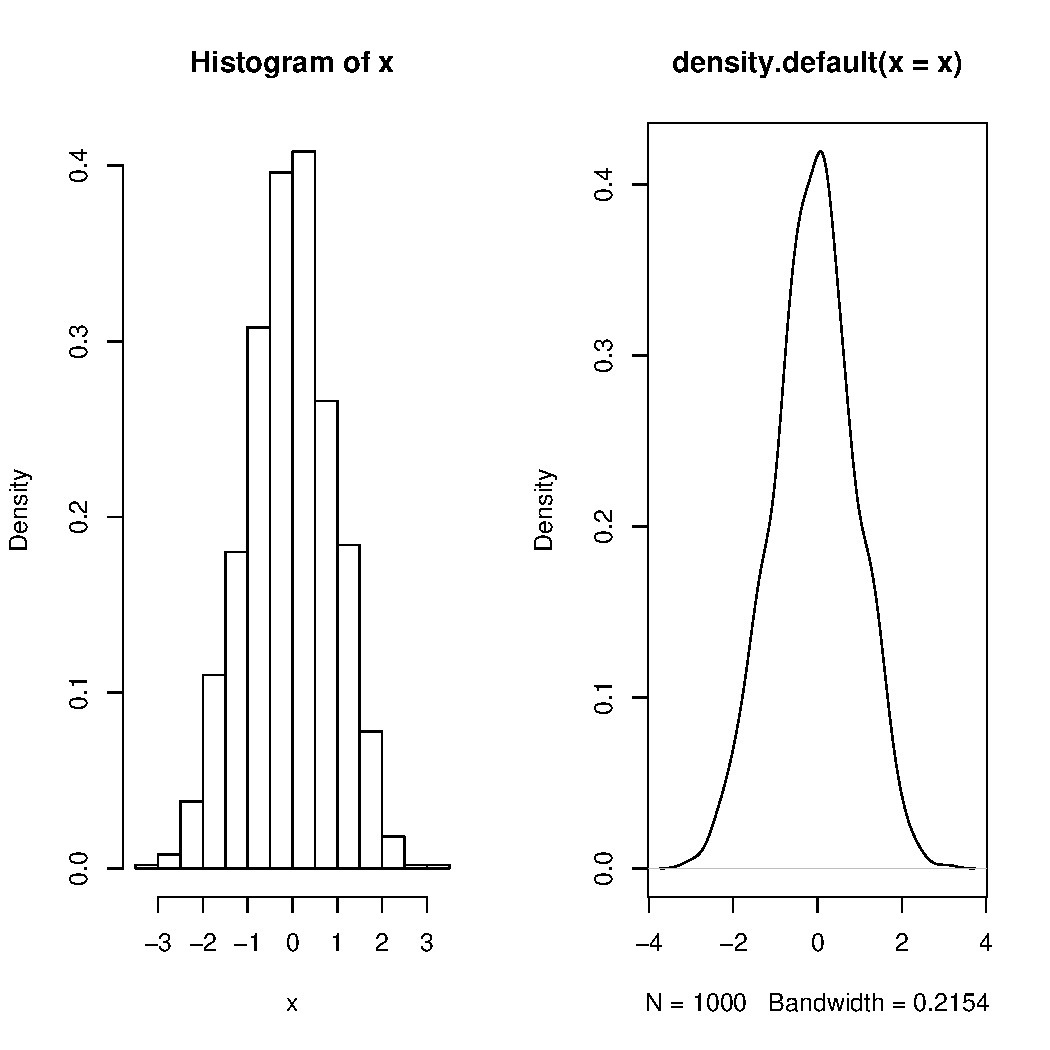
\includegraphics[height = 8.5cm, width = 15cm]{figure/viewport_demo_1.pdf}
  \caption{display the \texttt{grid} version of draw two plots into one overall graph by setting \texttt{par(mfrow())}. The left-plot is the histogram of observations generated by standard normal distribution, right-plot is the density plot of the observations}
  	\label{figure_4.1}
\end{center}
\end{figure}

\newpage
\begin{lstlisting}
grid.ls(viewports = TRUE)

 graphics-root
   graphics-inner
     graphics-figure-1
       graphics-plot-1-clip
         graphics-window-1-1
           graphics-plot-1-rect-1
           5
 graphics-root
   graphics-inner
     graphics-figure-2
       graphics-plot-2-clip
         graphics-window-2-1
           graphics-plot-2-lines-1
           5

\end{lstlisting}
% PerspWindow, 
The previous code used the \texttt{graphics} package to plot a histogram on the left and a density plot of a 
thousands of random observation generated by standard normal distribution. Then redraw the plot on \texttt{grid}. The grobs object and the veiwports are created. \\

The grobs object and the veiwports and been listed by \texttt{grid.ls()}. In the previous example, we can see that the contents(rectangles) of histogram were drawn in the viewports of \textit{graphics-inner::graphics-figure-1::graphics-plot-1-clip::graphics-window-1-1}. The density plot was drawn in the other viewports which is \textit{graphics-inner::graphics-figure-2::graphics-plot-2-clip::graphics-window-2-1}. Although it is completely different structure of the plot that was drawn by \texttt{graphics}, they are identical to each other.\\

To reproduce the same plots as \texttt{graphics}, we need to modify the \texttt{grid} structure of the plot so that it behaves identically to the plot that was drawn by \texttt{graphics}. In this example, the viewports need to be set in the same location and the same size as the \texttt{graphics} plot region, and also, the x-scale and y-scale of the viewports in \texttt{grid} need to be set the same user coordinates as in \texttt{graphics}.\\

\section{Integrate \texttt{persp()}}
The core of \texttt{gridGraphics} package provides some basic viewport structure to support the perspective plots(\texttt{persp()}), based on the gerneral plots that been drawn by \texttt{graphics}. However, there are some specific details that \texttt{gridGraphics} not fully supported. The following problems need to be solved before integrating \texttt{persp()} into the package:
\begin{itemize}
  \item{The viewport that \texttt{persp()} needs to be on}
  \item{The xcale and yscale need to be calcualted}
  \item{whether the clipping happens for every component when drawing}
\end{itemize}

It is not allowable to call \texttt{grid.newpage()} to create a new page for drawing a perspective plot since it will destory other feathers within the plot. For example, the points and lines added to perspective plot. These features will desappear when calling \texttt{grid.echo()} to reproduce the plot, since they are in a different viewport and the current graphics devices only contains the viewport that I created. Therefore, it is necessary to draw the perspective plot in the correct viewport.\\

The other problem that we may consider is the actual scale for the viewport, i.e. the x-scale and y-scale. Unfortunately, \texttt{gridGraphics} does no support the calculation for the actual limit of x and y since the other kinds of plot that \texttt{graphics} provides is in two dimension. The calculation of the limit of x and y is not as simple as \texttt{range(x)} or \texttt{range(y)}, because there is one more dimension of \texit{z}. And, the plot is drawn in a two-dimension graphics devices.\\

The final problem will be wether the clipping happeneds. More specifically, the different components of the perspective plot should be drawn in clipped region or non-clipped region. \\

The first problem can be solved by ...\\
% not sure how     dev.set(recordDev()) %par = currentPar(NULL) %dev.set(playDev()) works...

The limit of x and y will depend on the ratio of horizontal and verticle length of the current windows graphics devices. On \texttt{grid}, it is simple to track the actual length of the viewport in the current windows graphics devices. \\

The following exmple is calculating the verticle length and horizontal length of the viewport in current windows graphics devices. (See figure \ref{figure_4.2}) The dotted rectangle region is the viewport region that we focus on. As result, the verticle length of the viewport in current windows graphics devices in my PC is 5.16 inches, where the horizontal length is 5.76 inches. \\


\begin{Schunk}
\begin{Sinput}
> plot(cars$speed, cars$dist, col = 'orange', 
+      pch = 16, xlab = 'speed', ylab = 'dist')
> grid.echo()
> downViewport('graphics-plot-1')
> grid.rect(gp = gpar(col = 'red', lty = 12221, lwd = 2))
> convertX(unit(1.0, 'npc'), 'inches')
\end{Sinput}
\begin{Soutput}
[1] 5.76inches
\end{Soutput}
\begin{Sinput}
> convertY(unit(1.0, 'npc'), 'inches')
\end{Sinput}
\begin{Soutput}
[1] 5.16inches
\end{Soutput}
\end{Schunk}

\begin{figure}[h]
\begin{center}
  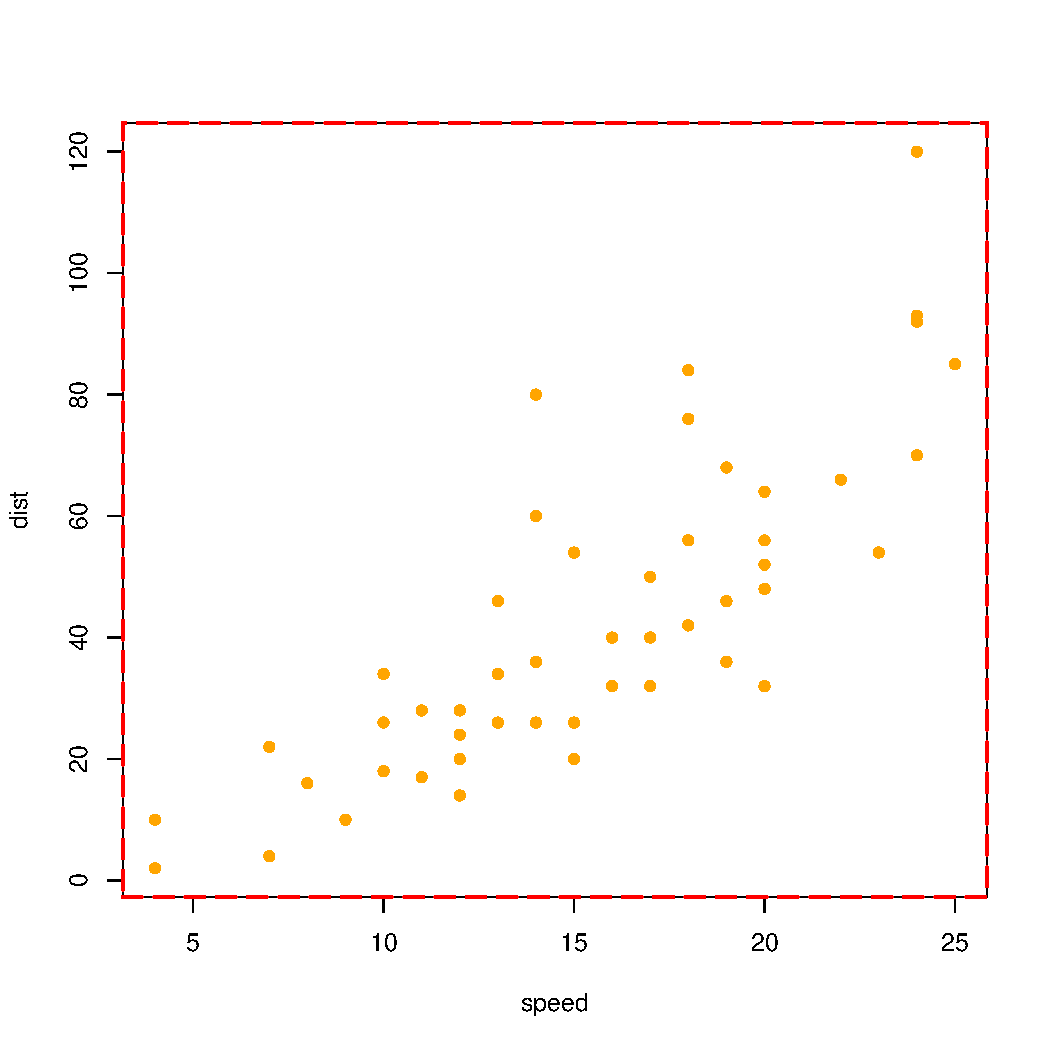
\includegraphics[height = 10cm, width = 10cm]{figure/gridGraphics_persp_demo_1.pdf}
  \caption{Used the example from chapter 2, calculate the actual verticle length and horizontal length of the viewport (the region of the red dotted line)}
  	\label{figure_4.2}
\end{center}
\end{figure}

\newpage
The idea of this example is that it is possible to track the actual vertical length and horizontal length by navigating to the specific viewport and record them. It leads to the solution of our second problem, first of all, we navigate to the viewport that has been drawn by \texttt{persp()}, calculate the limit of x and y base on the size of this viewport. Then we create another viewport (visible for other \texttt{gridGraphics} functions eg \texttt{lines()} and \texttt{points()}) that has the same location and the same size as the previous viewport. Then we modify the xscale and yscale from the new veiwport to be the limit of x and y that we calculated. Finally, the concepts of \texttt{persp()} will be drawn in this viewport. \\

\begin{Schunk}
\begin{Sinput}
> testPersp21(box = FALSE)
> usr = par('usr')
> rect(usr[1], usr[3], usr[2], usr[4], lty = 12221, lwd = 2, border = 'red')
> usr
> ## [1] -0.4555925  0.3807924 -0.5003499  0.3360350
> grid.echo()
> downViewport('graphics-window-1-0'); 
> grid.rect(gp = gpar(col = 'red', lty = 12221))
> c(current.viewport()$xscale, current.viewport()$yscale)
> ## [1] -0.04  1.04 -0.04  1.04
\end{Sinput}
\end{Schunk}

\begin{figure}[h]
\begin{center}
  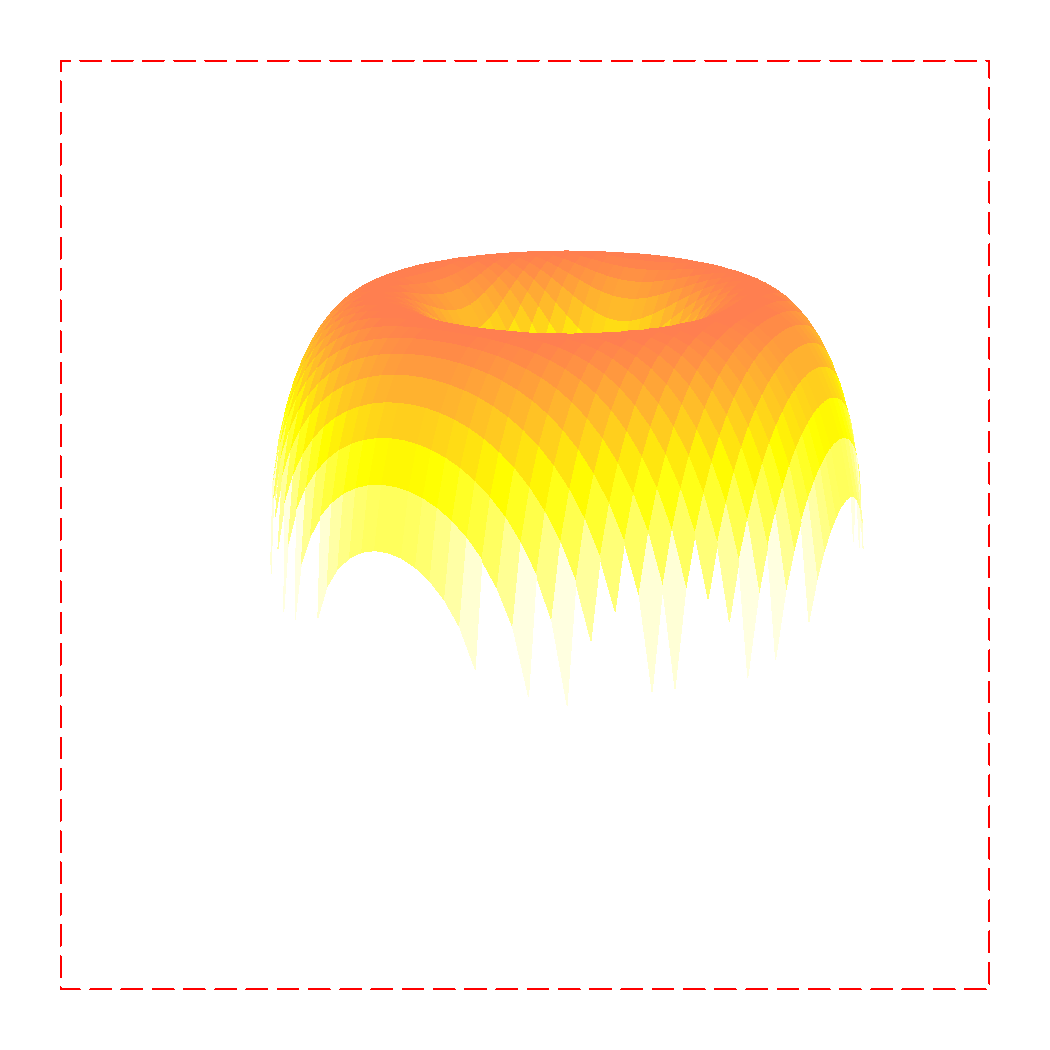
\includegraphics[height = 7cm, width = 7cm]{figure/gridGraphics_persp_demo_viewport_1.pdf}
  
\includegraphics[height = 7cm, width = 7cm]{figure/gridGraphics_persp_demo_viewport_2.pdf}
  \caption{A Torus been drawn by \texttt{persp()} on the left plot, the right plot tried to reproduce the \texttt{persp()}, because of the scale of the viewport is different to the limit, the Torus is been drawn on the bottom-left corner.}
  	\label{figure_4.3}
\end{center}
\end{figure}

Figure \ref{figure_4.3} shows a Torus drawn on the plot region. The red dotted rectangles indicate the plot region of \texttt{graphics}(left plot) and the viewport region for \texttt{grid}(right plot). Although the plot region is identical to the viewport region, the scales are different. The limit of x and y are $(-0.4555925,  0.3807924)$, $(-0.5003499,  0.3360350)$. The scale of x and y in the viewport region are $(-0.04,  1.04)$, $(-0.04,  1.04)$. Therefore, the scale needs to be moltified. \\

\begin{lstlisting}
## navigate to the viewport
depth = gotovp(TRUE) 
## calculate the limit of x and y
lim = PerspWindow(xr, yr, zr, trans, 'r')  
## create another viewport by using the limit that we just calculated
vp = viewport(0.5, 0.5, 1, 1, default.units = 'npc',
                xscale = lim[1:2], yscale = lim[3:4]) 
## back to the Root viewport
upViewport(depth)  
\end{lstlisting}
The code is creating a new temporary viewport which contains the true x scale and y scale prepared for drawing the perspective plot. The values for x scale and y scale are calculated by \texttt{PerspWindow()}. It will do the calculation by considering the 'actual' ratio of horizontal length and vertical length of the current graphics device, similar to the calculation of the \texttt{C} code does.\\
After we create the temporary viewport that contains the correct scale, then we added this viewport to the location of the tree which inside the viewport created by \texttt{gridGraphics}. That is, push temporary viewport inside the odd viewport. The Final step will be drawn the concepts within this viewport. To do that, we need to push a temporary viewport every time we drawn.\\ 
The following code is how does the surface of the plot is drawn internally.
\begin{lstlisting}
## navigate to the viewport which has the true limit of x and y
depth = gotovp(FALSE)
pushViewport(vp)
## draw the surface inside the viewport
DrawFacets(...)
## back to the Root viewport
upViewport()
upViewport(depth)
\end{lstlisting}

The next problem will be the merge the temporary viewport into the \texttt{gridGraphics} viewport tree to make sure all the features (such as points and lines are added afther perspective plots is drawn) are drawn in the correct viewport. Although the scales have been fixed, other features have no information about the temporary viewport. In the other word, these features are drawn in the viewport that \texttt{gridGraphics} creates rather than drawn in the temporary viewport. Figure \ref{figure_4.4} shows a Rosette shape ring is drawn above the surface of tour(left-plot). The left-plot is tried to reproduce a \texttt{grid} version by \texttt{grid.echo()}. Although the tour is drawn in the correct location, the Rosette shape ring appear on the bottom-left region of the plot(right-plot).

\begin{figure}[h]
\begin{center}
  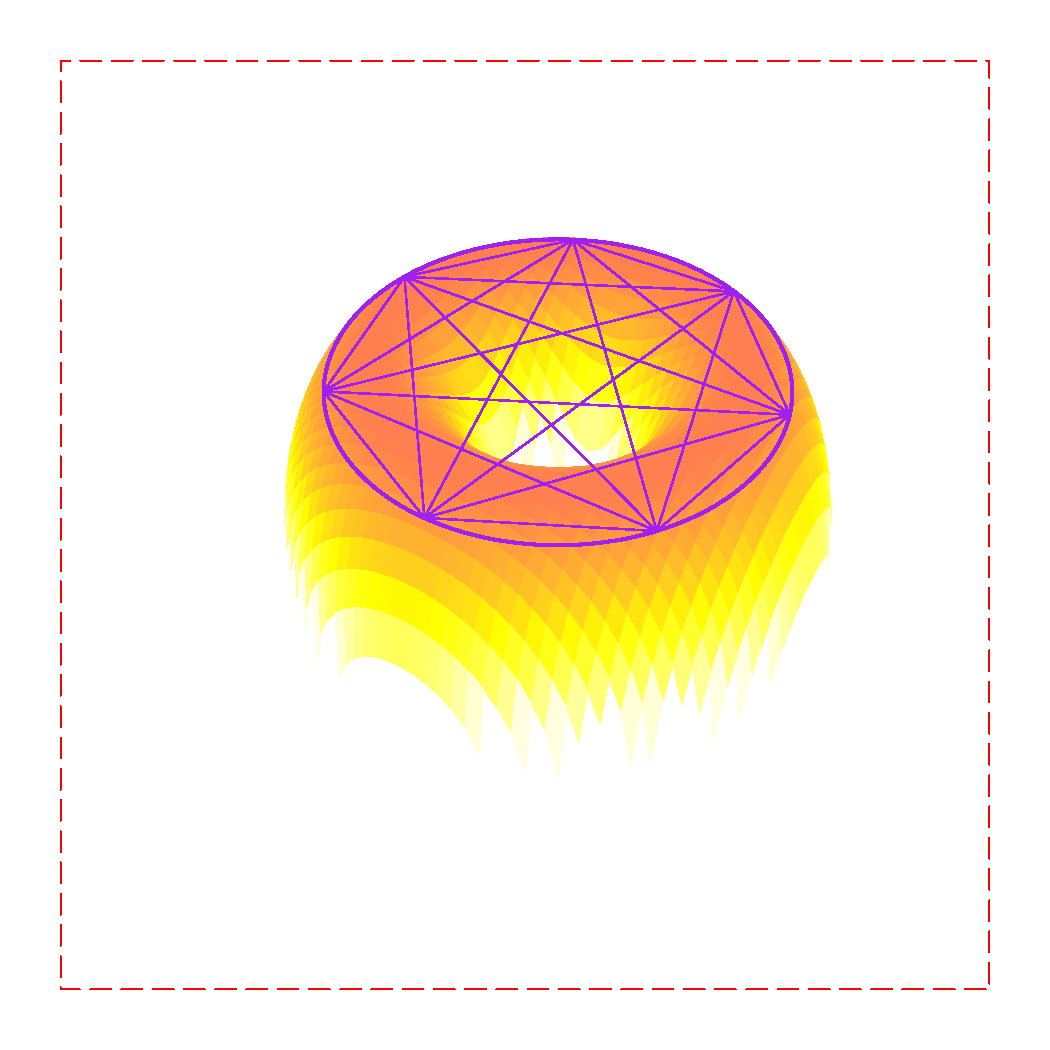
\includegraphics[height = 7cm, width = 7cm]{figure/gridGraphics_persp_demo_viewport2_1.pdf}
  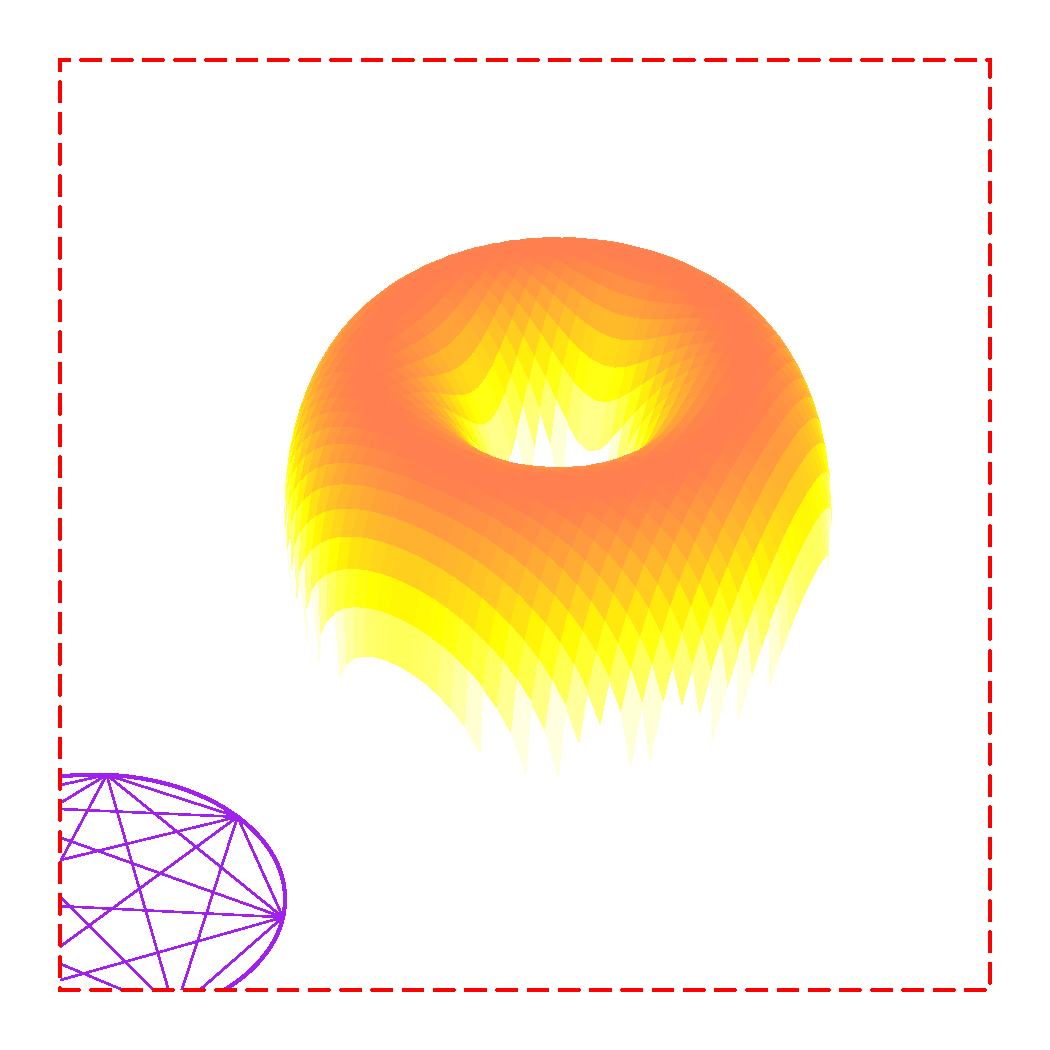
\includegraphics[height = 7cm, width = 7cm]{figure/gridGraphics_persp_demo_viewport2_2.pdf}
  \caption{A Rosette shape ring added to the tour(left-plot) on \texttt{graphics}, the right-plot reproduced the left-plot by \texttt{grid,echo()}. Althought the tour are identical, the Rosette shape ring is on the incorrect location.}
  	\label{figure_4.4}
\end{center}
\end{figure}

The final problem will be to decide whether allows the concepets are drawn outside the plot region or not . Figure \ref{figure_4.5} shows the previous tour surface draw over the limit of the box. The left-plot is drawn by \texttt{graphics} which is the behaviours that we need to reproduce on \texttt{grid}. In \texttt{persp()}, there are three concepts are been drawn, the surface of perspective plot, the box that contains the surface and the axes plus the labels of axes. By default, \texttt{graphics} draw the surface by setting \texttt{clipping = "on"}. On the other hand, the surface will not exceed the limit of the plot region. However, the box and the axes may be drawn outside the plot region if it is necessary. Alternatively, the right plot is drawn by \texttt{grid} which indicates compeletely result comparing with the left plot (the surface is drawn over the plot region but the axes is not drawn outside the plot region). Due to the perpose of this paper, it is necessary to make sure the plots as identical as possible.\\
In \texttt{grid}, it is possible to define a viewport that either 'cut' the concepts if they are excess the limit of the viewprot, or continuous draw them outside the viewport by setting the \texttt{clip} equal to be \texttt{"on"} or \texttt{"off"}.\\
The solution will be distinguished the clipping region for the concpets. Alternatively, the surface cannot excess the limit of the plot region therefore we need to "cut" the surface if it excesses the limit. On the oter hand, we drawn the surface in the \texttt{clip = "on"}'s viewport. The box and the axes (include the labels and the units) are drawn in the \texttt{clip = "off"}'s viewport.\\
Since \texttt{gridGraphics} package already setted up the clipping region, therefore it can be solved by navigating to the specific viewport and draw the concept of \texttt{persp()}. The following code is the action of solving this problem.
\begin{lstlisting}
...
## go to the viewport weather clip = 'off'
depth = gotovp(TRUE)
## draw the axes
PerspAxes(...)
upViewport(depth)
...
## go to the viewport weather clip = 'off'
depth = gotovp(TRUE)
## draw the Box
EdgeDone = PerspBox(0, xr, yr, zr, EdgeDone, trans, 1, lwd)
upViewport(depth)
...
## go to the viewport weather clip = 'on'
depth = gotovp(FALSE)
## draw the surface
DrawFacets(...)
upViewport(depth)
...
\end{lstlisting}\\

\begin{figure}[h]
\begin{center}
  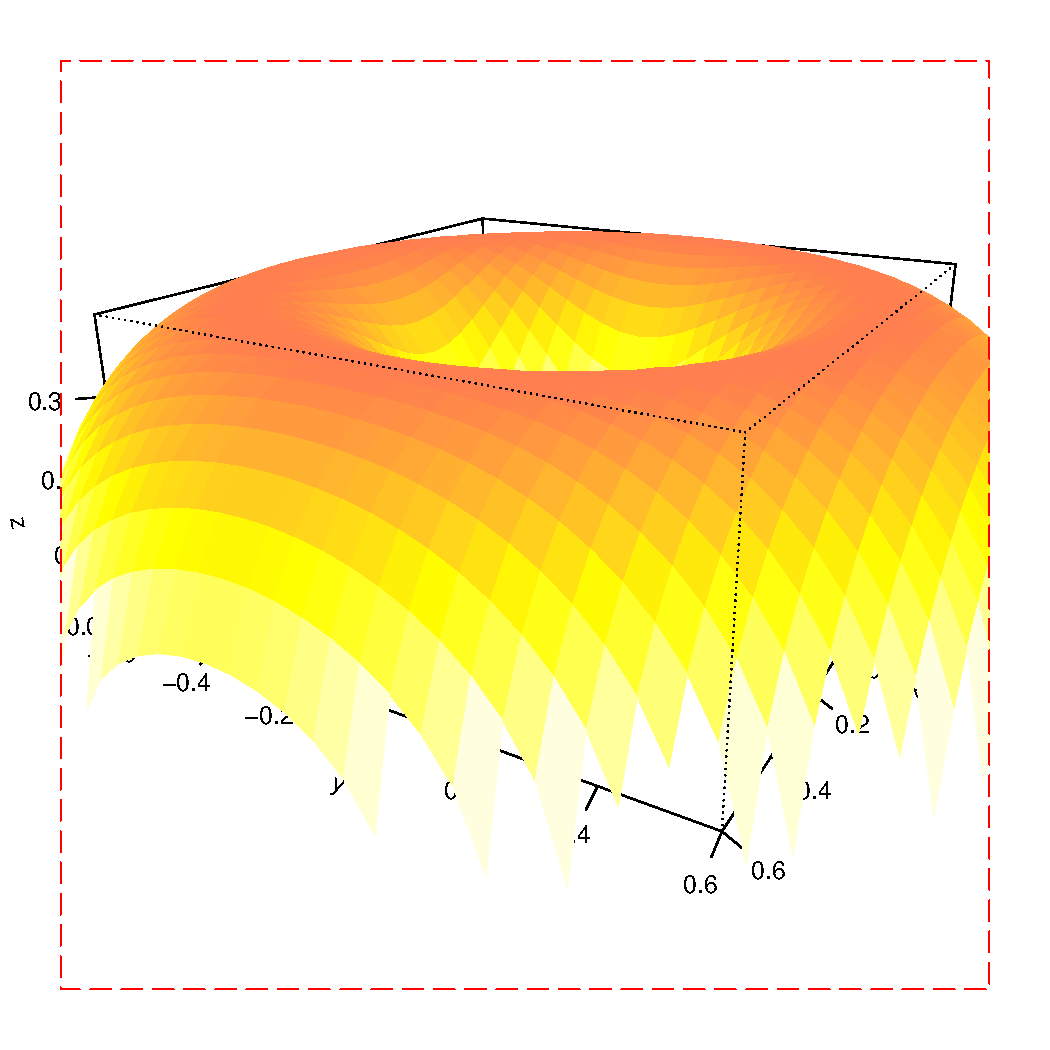
\includegraphics[height = 7cm, width = 7cm]{figure/gridGraphics_persp_demo_viewport3_1.pdf}
  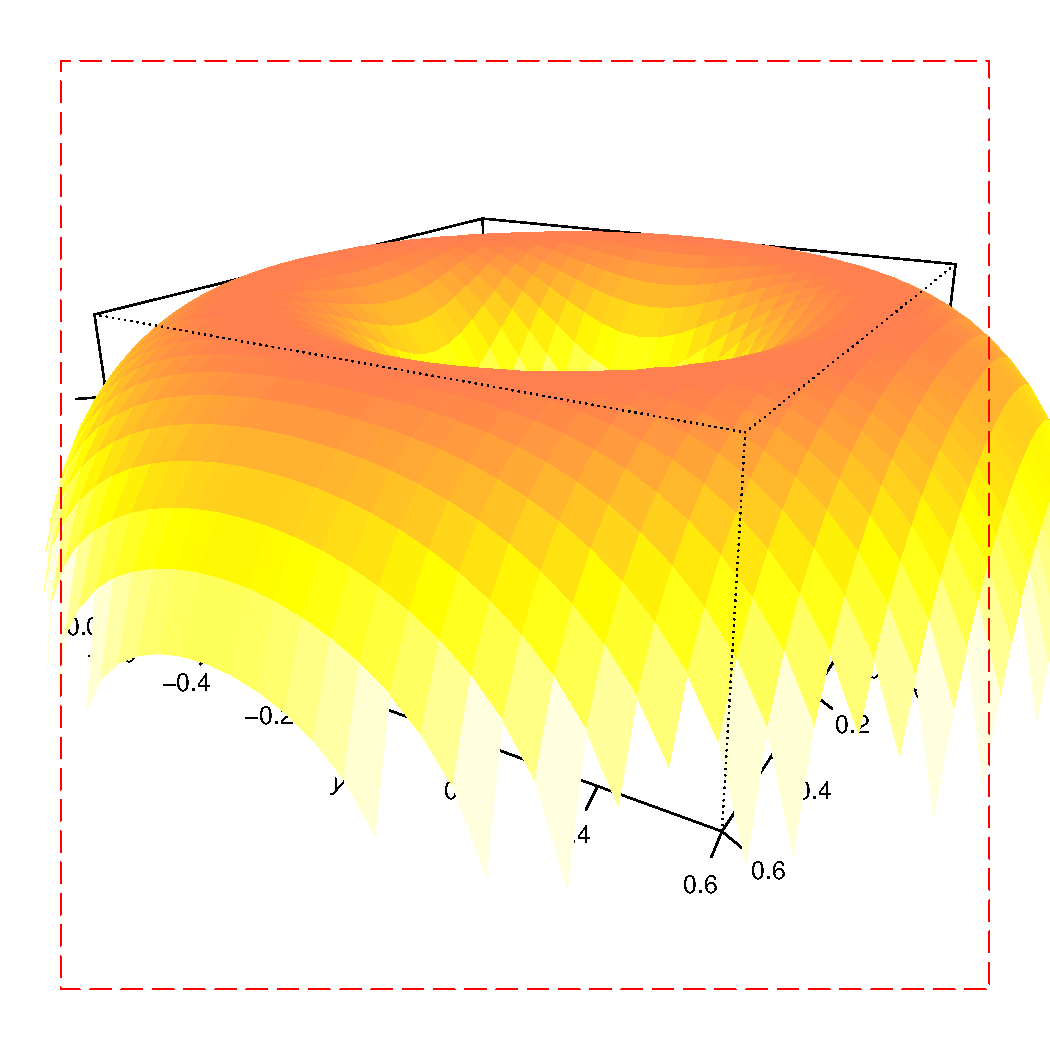
\includegraphics[height = 7cm, width = 7cm]{figure/gridGraphics_persp_demo_viewport3_2.pdf}
  \caption{A \texttt{graphics} \texttt{persp()} is drawn at the left. The red regions are the plot region for \texttt{graphics}(left plot) and the viewport region for \texttt{grid}(right plot). Clearly, the right plot is tried to reproduce the left plot, but the surface is not allowed excess the limit of the viewport, but the axes label and units are needs to be drawn even excess the limit.}
  	\label{figure_4.5}
\end{center}
\end{figure}



\section{Integrate \texttt{filled.contour()}}
Unlike \texttt{persp()}, \texttt{filled.contour()} is "made up" by multiple plots in one plot region. \texttt{gridGraphics} package will take care about most of the simple plots (such as the levels bar on the right-hand side of the plot, the titles, and the axes). (See figure \ref{figure_1.3} or figure \ref{figure_3.6}).\\

\texttt{gridGraphics} fully convert the layout of \texttt{filled.contour()} to the viewport structure of \texttt{grid}, therefore we do not need to build or modify the viewports. However, it is necessary to "move" the filled contours into the correct location with the correct scale. On the other hand, we need to draw the filled contours in the correct viewport.\\

In section 3.2, we discussed how a Filled Contour Plot been drawn by the \texttt{filled.contour()}. More specifically, we only figure out who we drawn the main filled contour, but we still do not know how we display it. The next task is to display Filled Contour Plot in the correct location. Figure \ref{figure_4.6} shows the top-left is the contents of \texttt{filled.contour()}, which redrawn by using \texttt{grid} package. The red dotted rectangle is the viewport region. The next step is fill the blank region (top-right plot) by the top-left plot. The solution is similar to the first step of integrating \texttt{persp()}, that is, navigating to the correct viewport region and then drawn the filled contour. The following code is the solution in action.

\begin{lstlisting}
...
## navigating to the correct viewport
depth = gotovp(TRUE)
## actual drawing
grid.polygon(...)
## reset
upViewport(depth)
...
\end{lstlisting}


\begin{figure}[h]
\begin{center}
  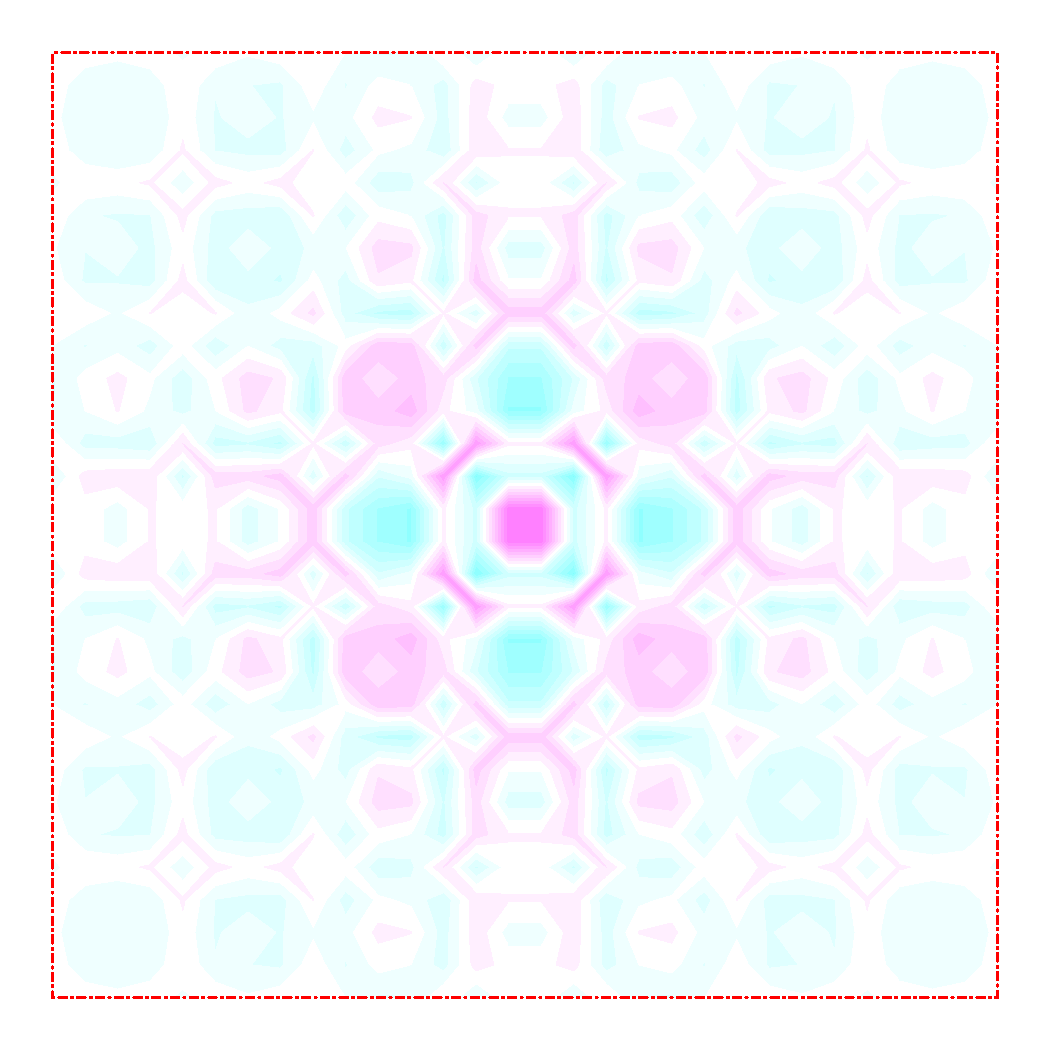
\includegraphics[height = 7cm, width = 7cm]{figure/filledContour_origin_02.pdf}
  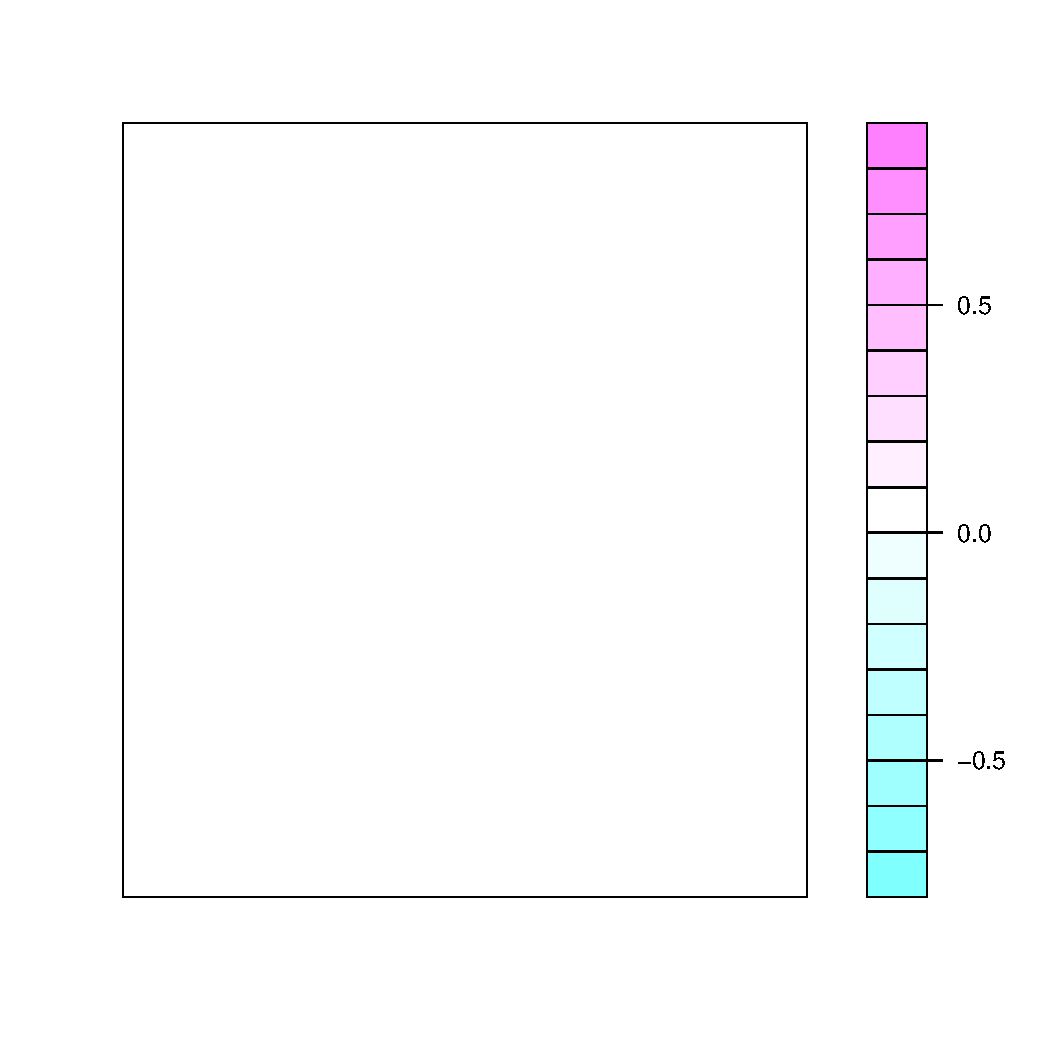
\includegraphics[height = 7cm, width = 8cm]{figure/filledContour_origin_03.pdf}
  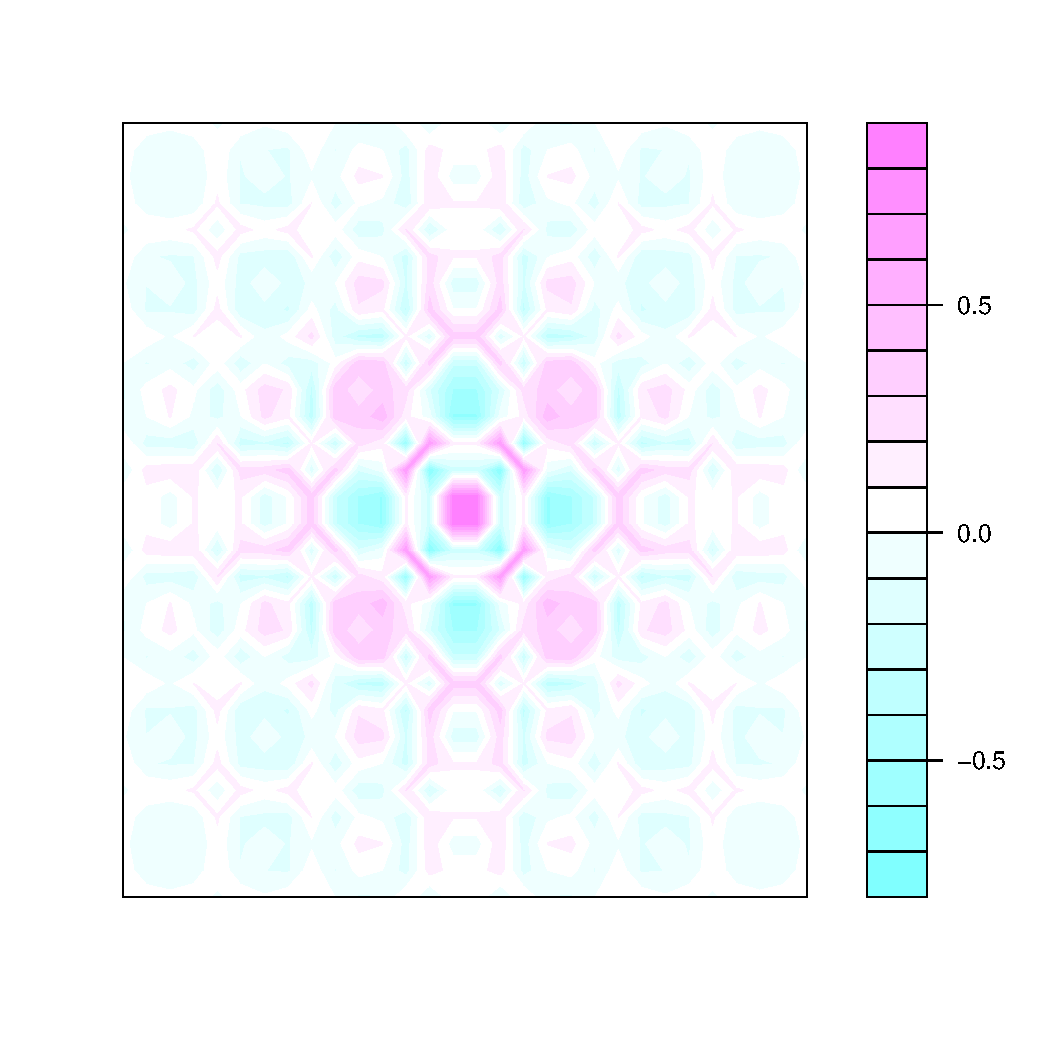
\includegraphics[height = 7cm, width = 8cm]{figure/filledContour_origin_01.pdf}

  \caption{The top-left filled contour are plotted by \texttt{grid}, top-right plot is the failed reproduce the \texttt{filled.contour()} by \texttt{grid.echo()} at the original state, and the bottom-center plot is the success reproduce the \texttt{filled.contour()} by \texttt{grid.echo()} after integrated to the \texttt{gridGraphics} package.}
  	\label{figure_4.6}
\end{center}
\end{figure}


\chapter{Testing}
The aim of this paper is to redraw Perspective Plots and Level (Contour) Plots using the \texttt{grid} package with an identical result to the \texttt{graphics} package. Every plot drawn by \texttt{grid} graphics should be not only identical to \texttt{graphics} by human eye, but also the machine 'thinks' they are identical.\\

However, there are some tiny differences which cannot distinguish by human eye, for example, the color are differences at one pixel between two plots, or the colors of few area have one unit difference on red Channel distortion compare to the other plot. Therefore, we need software to detect those tiny differences.\\

\textbf{ImageMagick} is the software that can be used for the comparison in this paper, it can create, edit, compose, or convert bitmap images and read and write images in a variety of formats (over 200). The features used in this paper is \texttt{compare}, which is a program to mathematically and visually annotate the difference between an image and its reconstruction.\\

The following example (see figure \ref{chapter5.1}) are drawn two rotated sinc function, where the colors of the surface are close to each other and cannot be distinguish by human eyes. However, there is a difference for the colors, the top-left plot ($rgb = 211, 182, 255$) has one color pixel higher on red channel than the right-plot ($rgb = 210, 182, 255$). The bottom plot shows the difference, the region filled by red color is the difference, which is true because the color of the surface is different, the box and labels which have lighter color because they are mathematically and visually identical to each other. \\

\begin{figure}[h]
\begin{center}
  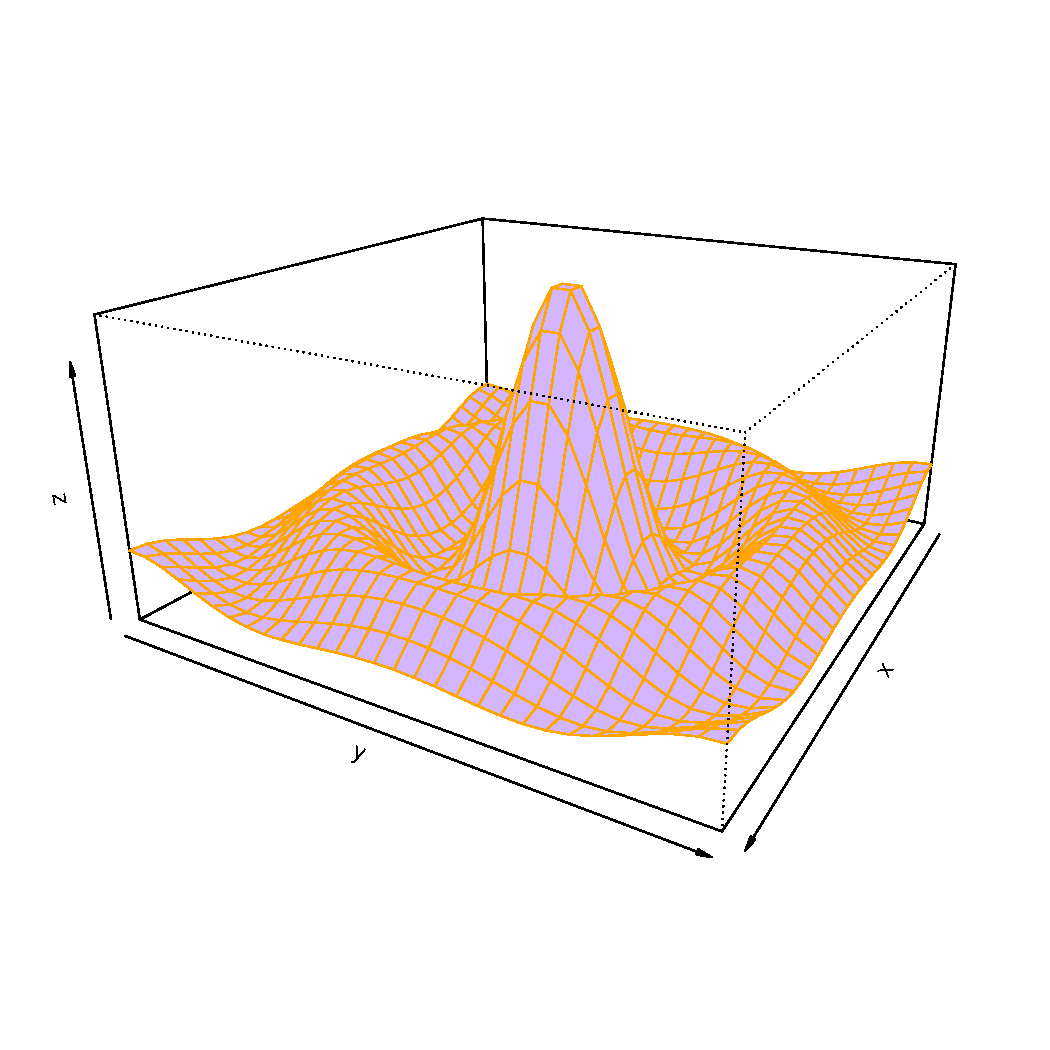
\includegraphics[height = 7cm, width = 7cm]{figure/Chapter5_example_01.pdf}
  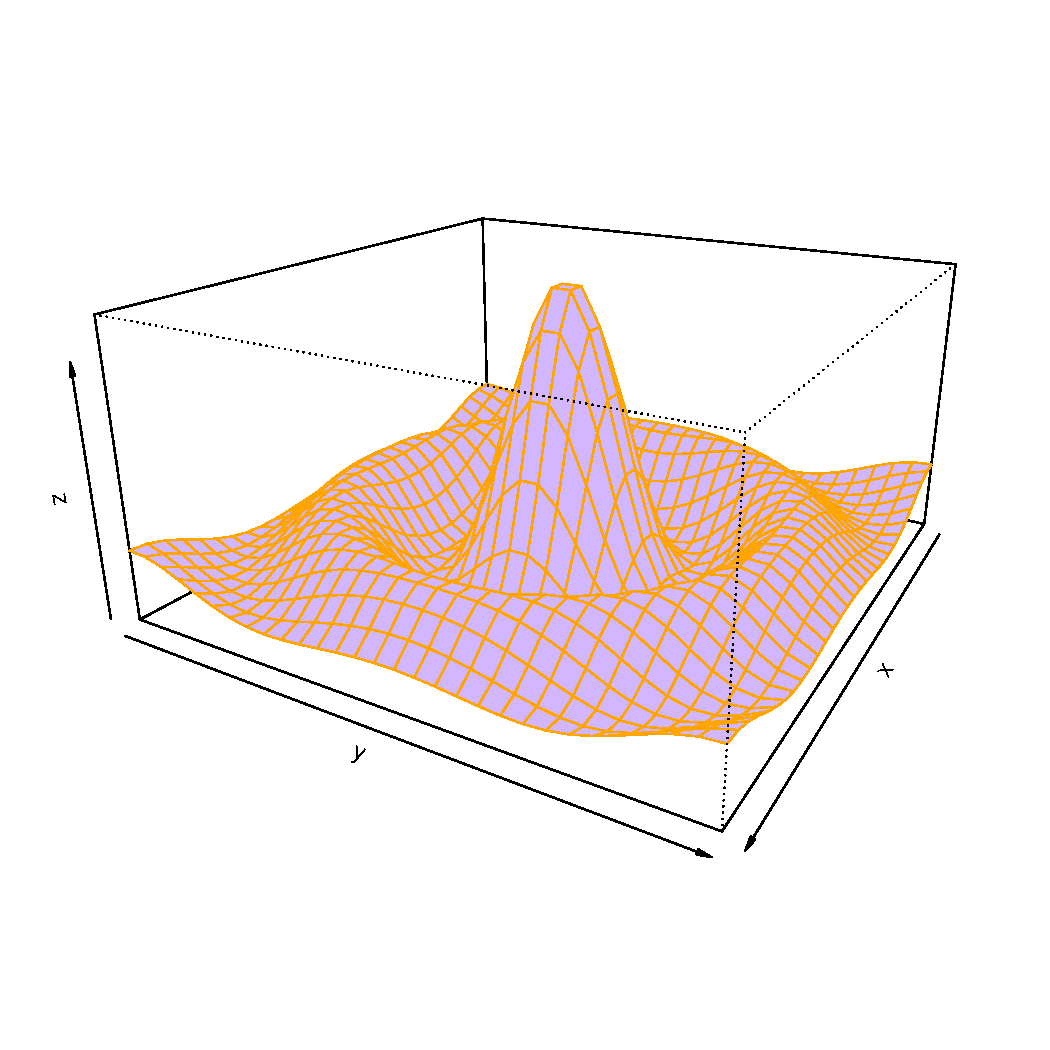
\includegraphics[height = 7cm, width = 7cm]{figure/Chapter5_example_02.pdf}
  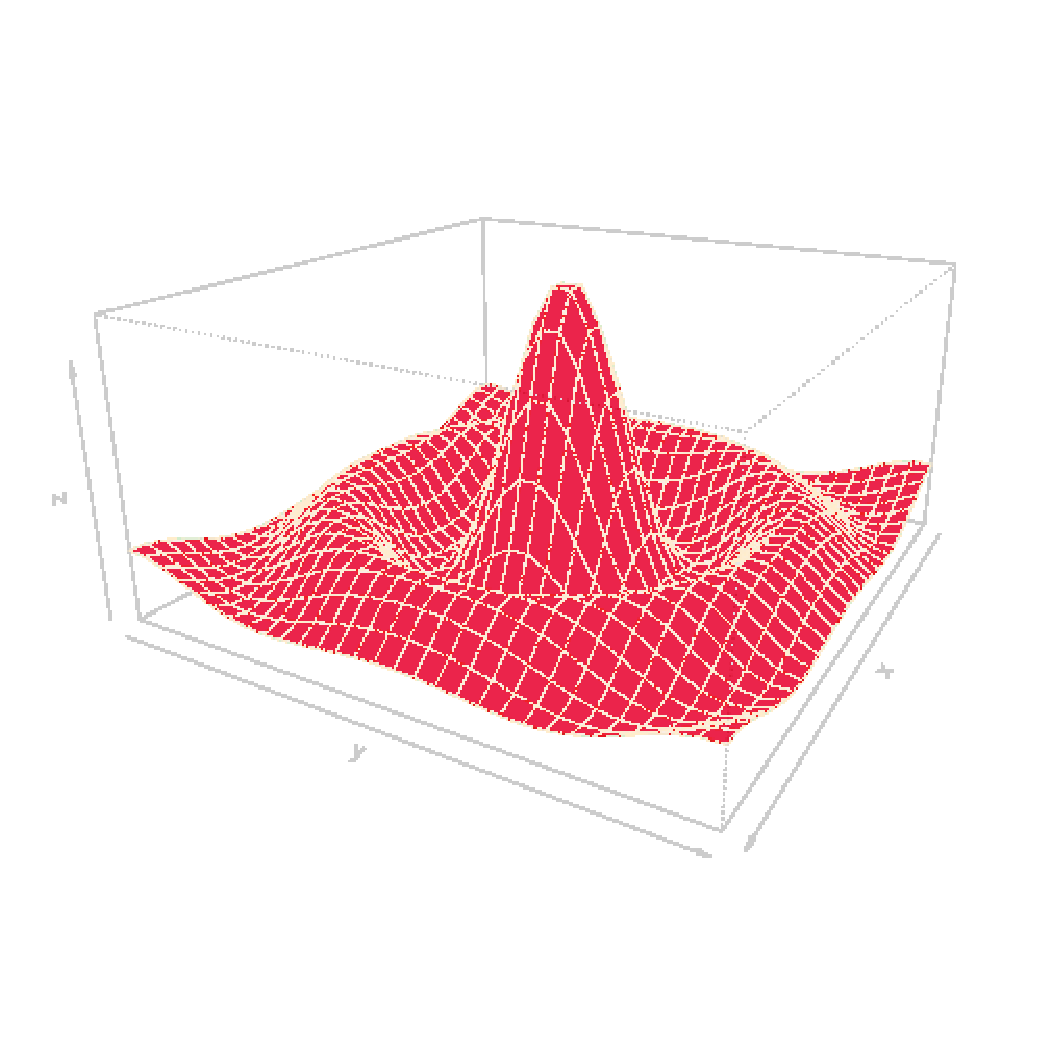
\includegraphics[height = 7cm, width = 7cm]{figure/Chapter5_example_03.pdf}

  \caption{The top-left plot looks identical to the plot at top-right by human eyes, however, there is a tiny difference at the color of the surface, which been detected by the software, the red color indicated the difference.}
  	\label{chapter5.1}
\end{center}
\end{figure}

The following figure shows the test that built in the \texttt{gridGraphics} package. In this section, we only show the different plot. The \texttt{graphics} and \texttt{grid} plots are in \ref{}.\\
% no image return when they are identical



\chapter{Example}
\texttt{persp()} and \texttt{filled.contour()} are now supported by \texttt{gridGraphics}. This means most of the plots that drawn by \texttt{persp()} and \texttt{filled.contour()} by \texttt{graphics} package now is able to reproduce by \texttt{grid.echo()} on \texttt{grid}. The advantage of \texttt{grid} is \texttt{grid} is more flexible than \texttt{graphics}. For example, a plot drawn by \texttt{grid} can record the viewport structure and we may draw and edit any plot features within different viewport easily. However, a plot drawn by \texttt{graphics} may not been edited easily.\\

One simple example is drawing some points in the plot region. (See figure \ref{Example_6.0}.) On the left figure, some random points are drawn by \texttt{graphics} package. However, it is not allowable for us to moltify the feature of the existence plot (eg, the style or the color of the points). The left plot is some random points are drawn in the plot with \texttt{pch = 12} and \texttt{col = "orange"}, where the right plot are draw the same points but with different color and style (\texttt{pch = 16} and \texttt{col = "red"}). Therefore, the right plot look quite rare.\\
%change the example?

One approximate solution to change the style and color of the points in the left plot of figure \ref{Example_6.0} is that redrawn the points with new style and color, rather than add the same points with different style and color.\\

The other solution will be convert the plot from \texttt{graphics} into \texttt{grid} by using the \texttt{gridGraphics} package, then use \texttt{grid.edit()} to modify the color and the style of the current plot.\\

\begin{figure}[h]
\begin{center}
  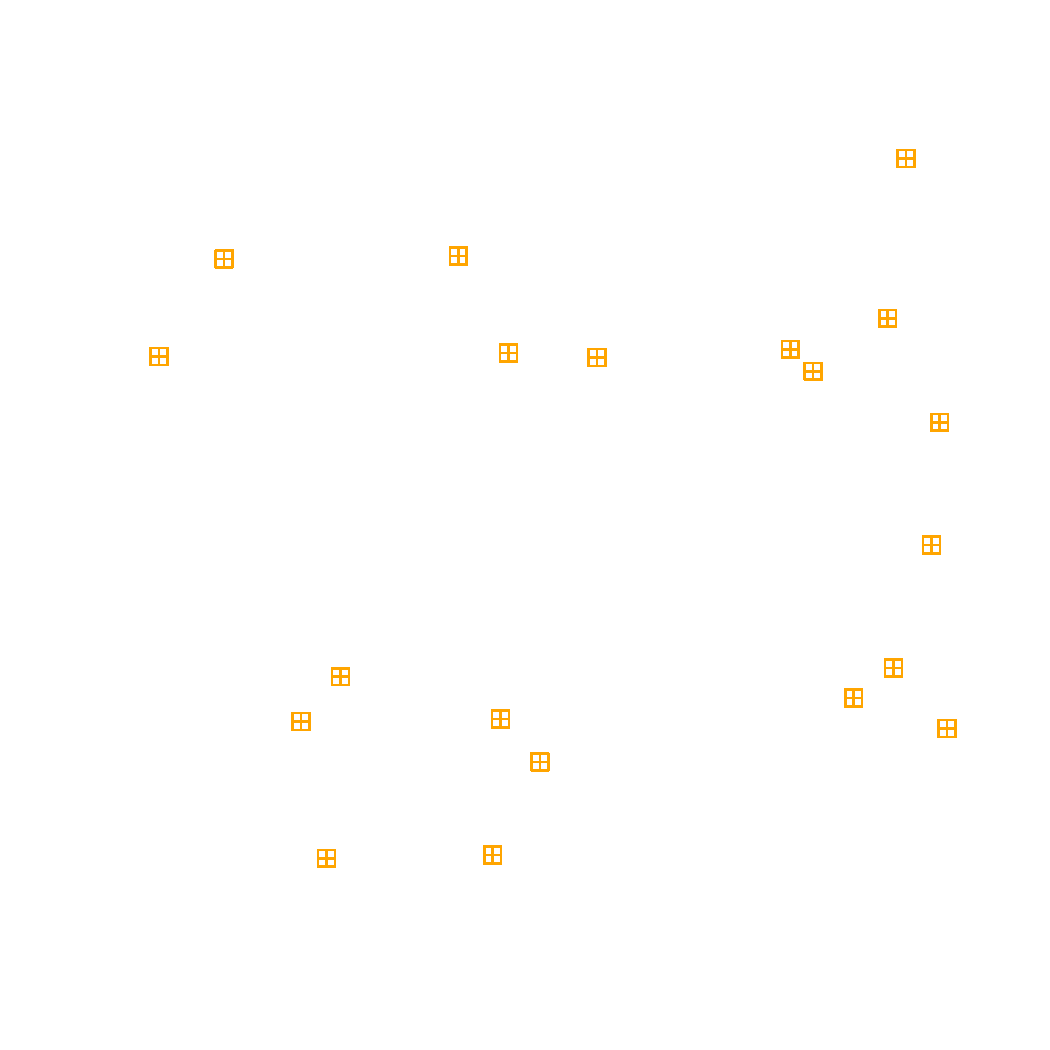
\includegraphics[height = 7cm, width = 7cm]{figure/Chapter6_example_1.pdf}
  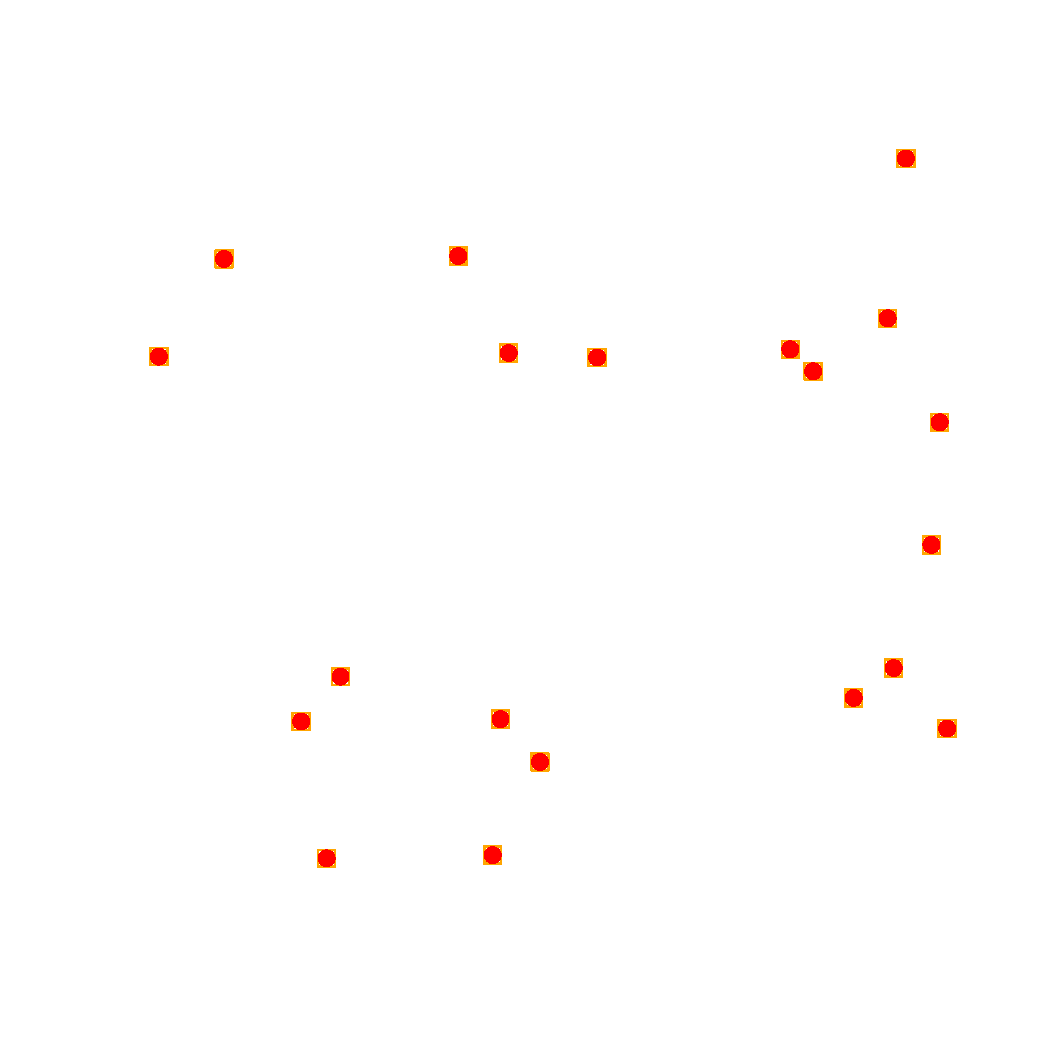
\includegraphics[height = 7cm, width = 8cm]{figure/Chapter6_example_2.pdf}
  \caption{..}
  	\label{Example_6.0}
\end{center}
\end{figure}

\section{Example to solution}
The \texttt{persp()} and \texttt{filled.contour()} are now can been edit more easily since they are integraded to \texttt{gridGraphics}. On the other hand, they are now available been drawn on \texttt{grid}.\\

An other Torus shape is drawn by \texttt{graphics} (See figure \ref{Example_6.3}), it has been redrawn on \texttt{grid} by \texttt{grid.echo()} and then we can listing the grobs of this plot. Since we are only drawing the surface, and the surface is formed by polygons. Then we can modify the features of the polygons easily by using \texttt{grid.edit}. In this example, we changed the white color (with opacity is 0) to purple (with opacity is 0.3).\\


\begin{Schunk}
\begin{Sinput}
> Torus_shape(col = 'NA', border = 'gray', box = FALSE)
> grid.echo()
> grid.ls()
\end{Sinput}
\begin{Soutput}
polygon
\end{Soutput}
\begin{Sinput}
> newCol = rgb(160/255, 32/255, 240/255, alpha = 0.3)
> grid.edit('polygon', gp = gpar(fill = newCol))
\end{Sinput}
\end{Schunk}

\begin{figure}[h]
\begin{center}
  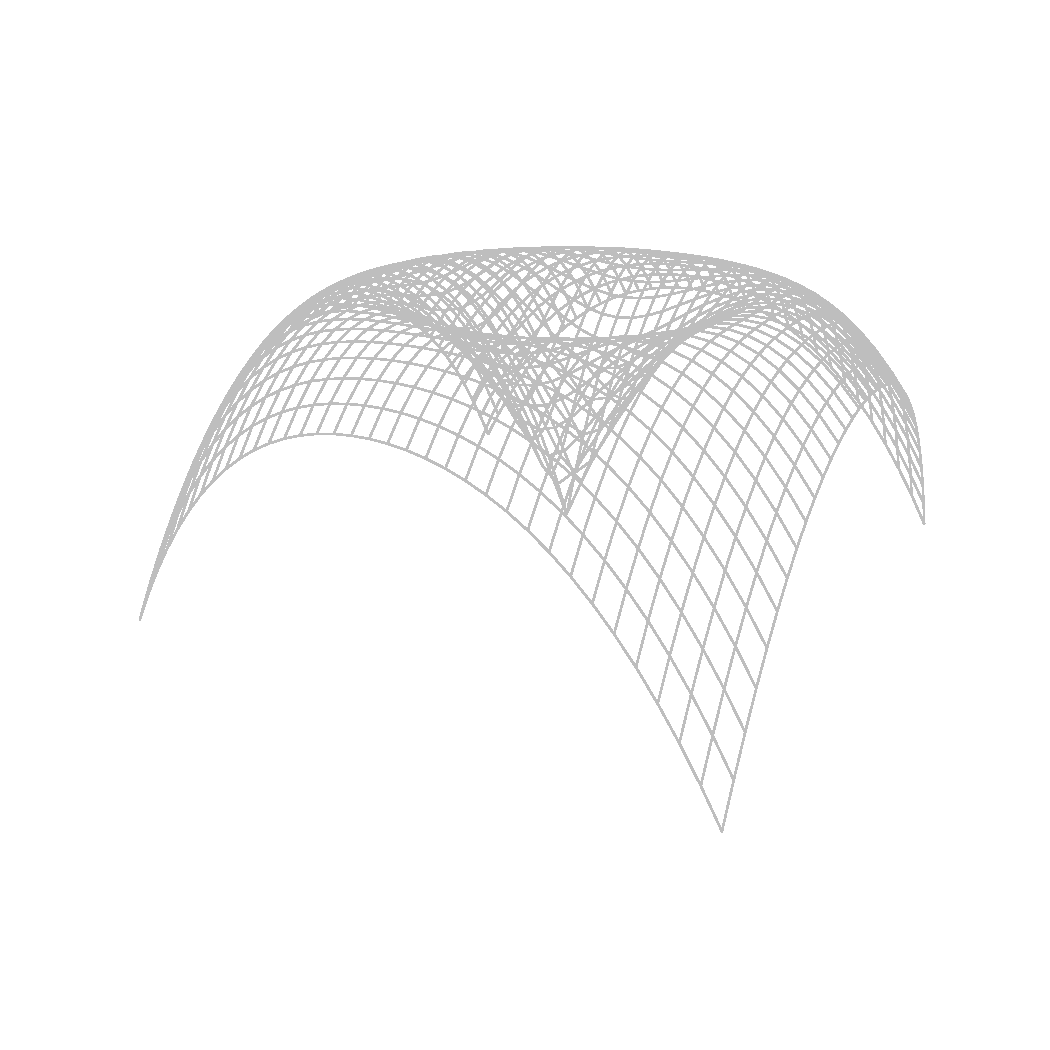
\includegraphics[height = 7cm, width = 7cm]{figure/Chapter6_example_1_2.pdf}
  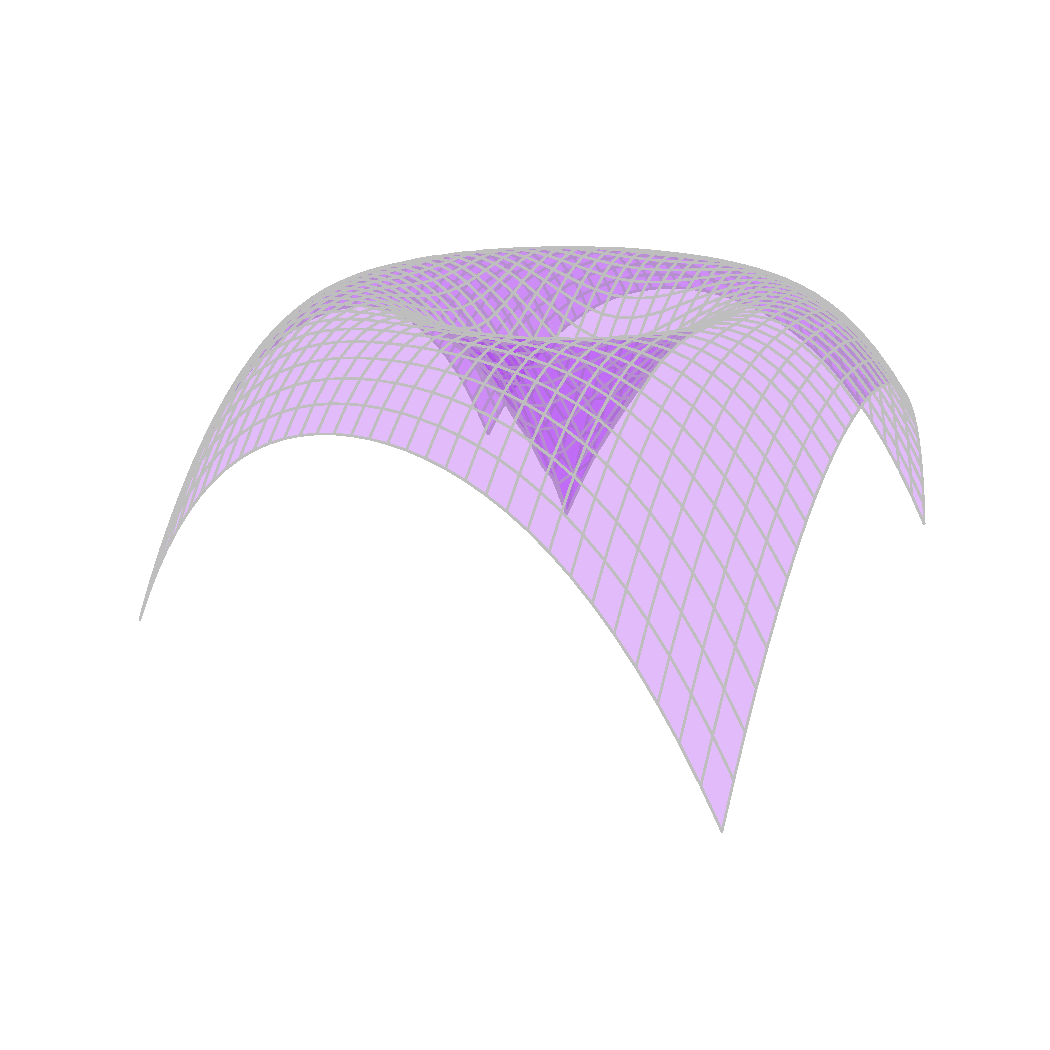
\includegraphics[height = 7cm, width = 8cm]{figure/Chapter6_example_1_3.pdf}
  \caption{The left plot is drawn by \texttt{graphics}, where the right plot is been drawn by redrawn the left plot on grid (\texttt{grid.echo()}) and then moltify the colors by \texttt{grid.edit()}}
  	\label{Example_6.3}
\end{center}
\end{figure}


\begin{Schunk}
\begin{Sinput}
> f8()
> grid.echo()
> grid.ls()
\end{Sinput}
\begin{Soutput}
graphics-plot-1-rect-1
graphics-plot-1-box-1
GRID.polygon.4
\end{Soutput}
\begin{Sinput}
> ## add color to the line of every polygons
> grid.edit(grid.ls(print = FALSE)$name[3], gp = gpar(col = 'white', lty = 1122))
\end{Sinput}
\end{Schunk}



\begin{figure}[h]
\begin{center}
  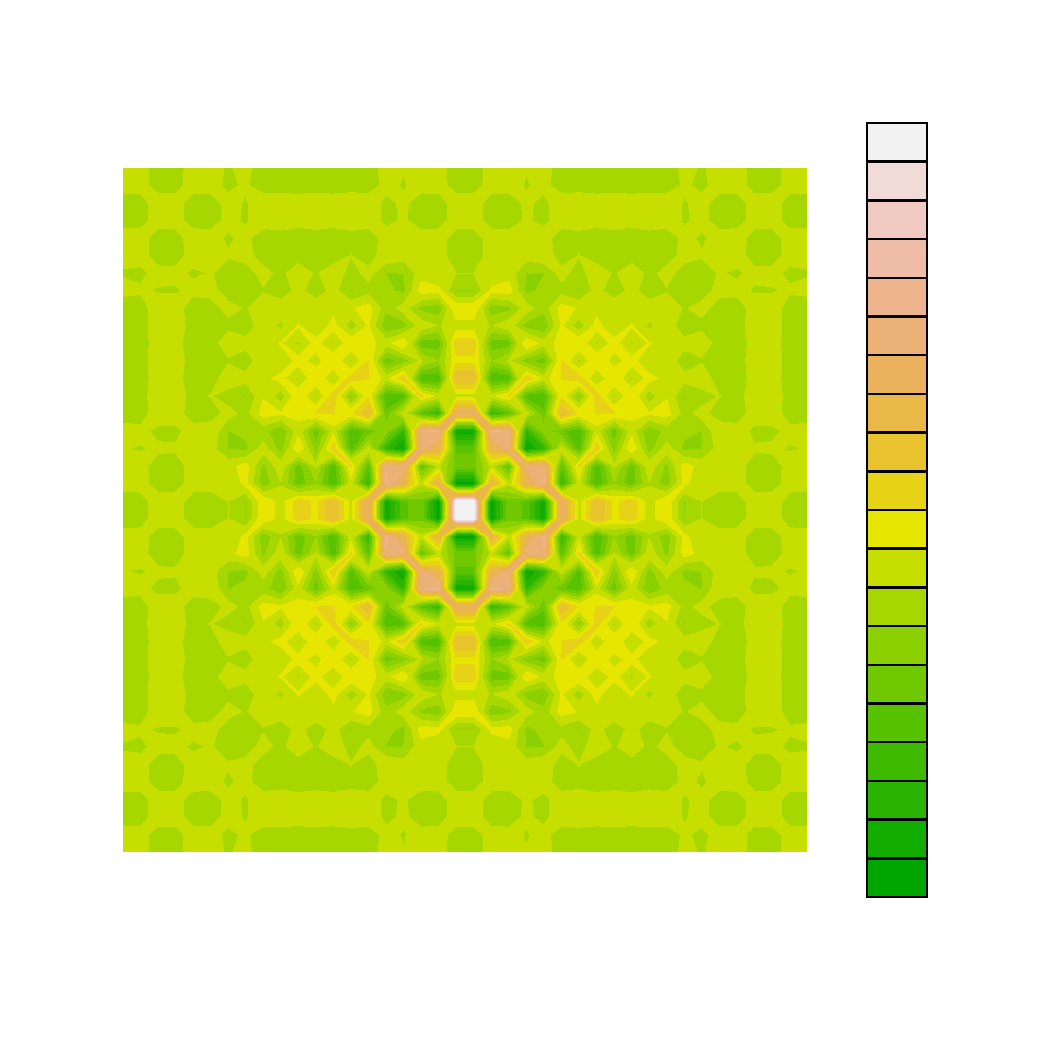
\includegraphics[height = 7cm, width = 7cm]{figure/Chapter6_example_2_2.pdf}
  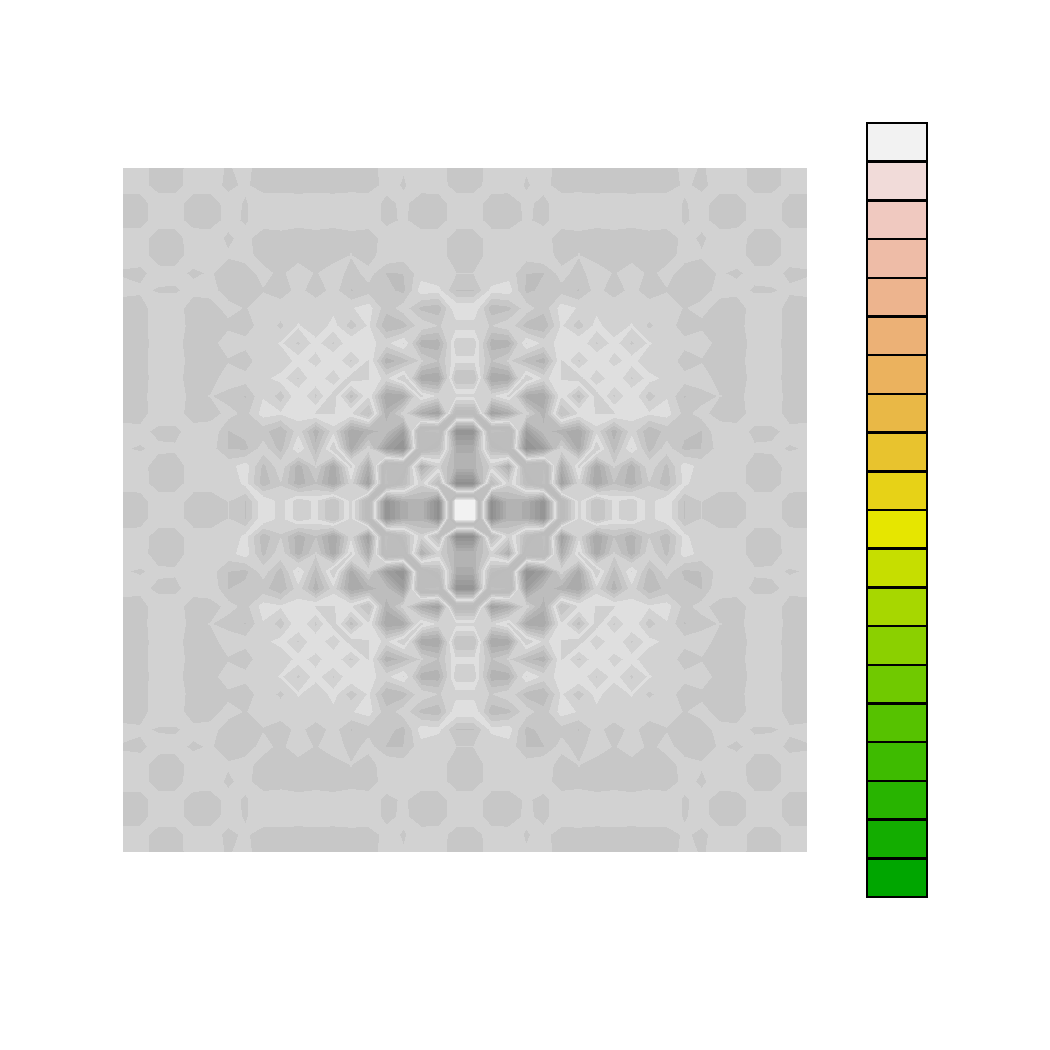
\includegraphics[height = 7cm, width = 7cm]{figure/Chapter6_example_2_3.pdf}
  \caption{The left plot is drawn by \texttt{graphics}, where the right plot is been drawn by redrawn the left plot on grid (\texttt{grid.echo()}) and then modify the colors by \texttt{grid.edit()}}
  	\label{Example_6.1}
\end{center}
\end{figure}

\newpage
\section{An advance example}
In \texttt{graphics} package it is very normal to draw two or more plots in the plot region. However, it is not allowable to combind the \texttt{filled.contour()} with any other kind of plots together within one plot region, because \texttt{filled.contour()} will create the layout itself when it been called. Therefore, even we specify a layout before plotting, the \texttt{filled.contour()} will overwrite the layout.\\

The viewport structures of \texttt{grid} provides more flexible than the layout of \texttt{graphics}, which allows us draw any other plots with \texttt{filled.contour()} within in one plot region. The idea will be create a viewport before drawing any plots (said root viewport), then push a viewport within the Root viewport for drawing a grid version of \texttt{filled.contour()} so that the \texttt{filled.contour()} only modify the structure of its own viewport but not overwriting the Root viewport. On the other hand, drawing one or more plot combine with \texttt{filled.contour()} is allowable on \texttt{grid}.\\
\begin{figure}[H]
\begin{center}
  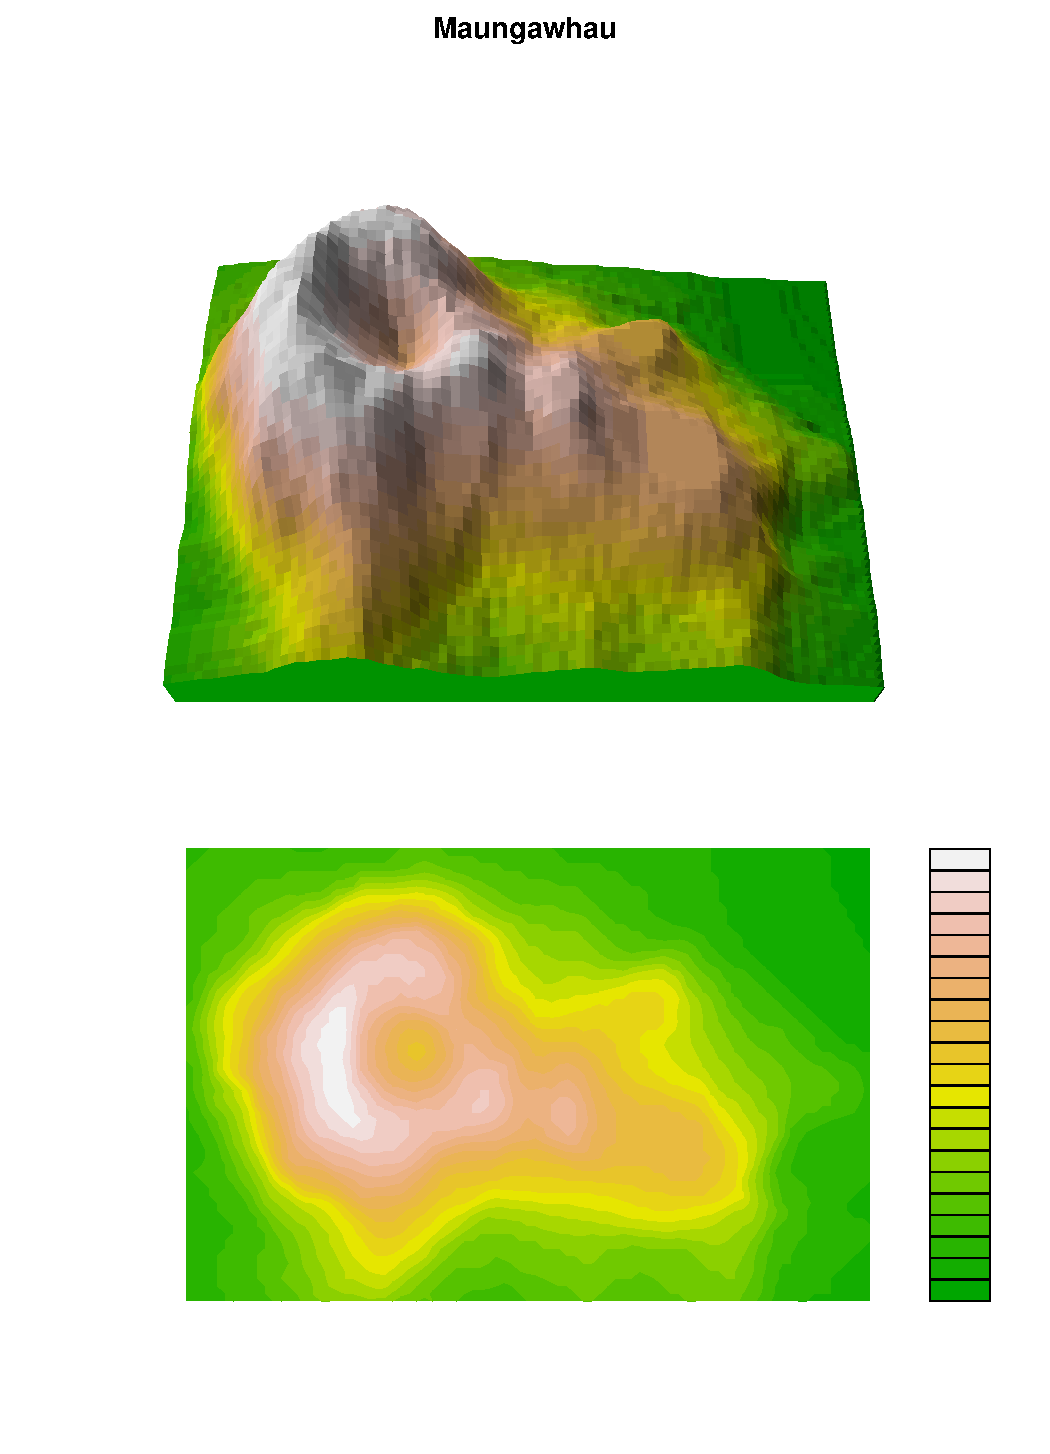
\includegraphics[height = 16cm, width = 12cm]{figure/Chapter6_example_3_1.pdf}
  \caption{The top plot shows the shape of Maungawhau volcano, where the bottom figure shows the level contour (i.e. the height)}
  	\label{Example_6.2.1}
\end{center}
\end{figure}

\newpage
\section{A more advance example}
Another benefit that \texttt{grid} provides is we can convert the graphics drawn with package \texttt{grid} to SVG format by the \texttt{gridSVG} package.
SVG (Scalable Vector Graphics) is a two-dimensional vector image format with XML-based. A SVG format graphics can support for interactivity and animation which most of the \texttt{R} graphics system is not supported or it is difficult achieve by \texttt{R} graphics system.\\

In this example, we are going through animation of the following action.
\begin{itemize}
  \item Changing the color of the surface
  \item Changing the opacity of the surface
  \item Shading the surface
  \item Highlighting the specific fragment of the surface and showing its z-value  
\end{itemize}

\subsubsection*{Animation of Changing the color of the surface}
The figure \ref{Example_6.3.1} shows the color of the sinc surface changing from light-yellow(left plot) to orange-red(right plot). The middle plot is captured during the animation. 
\begin{figure}[h]
\begin{center}
  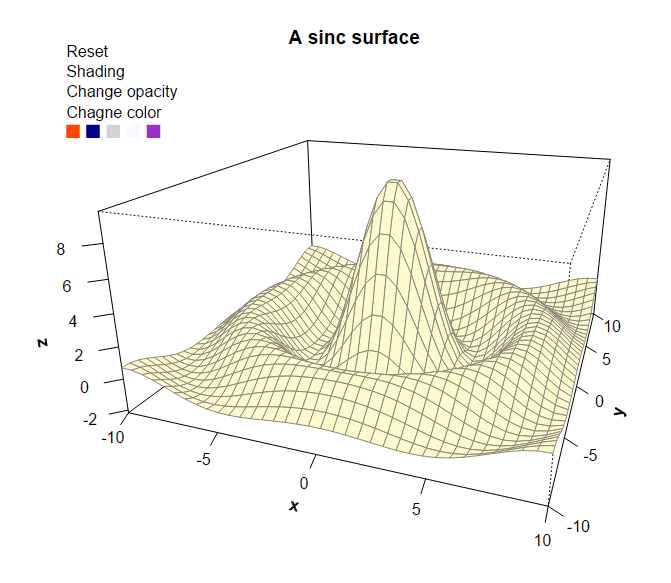
\includegraphics[height = 5cm, width = 5cm]{figure/svg/origin_1.PNG}
  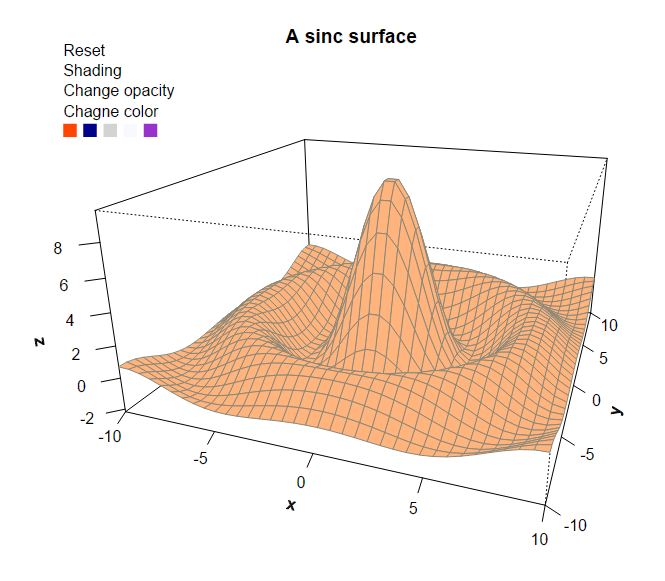
\includegraphics[height = 5cm, width = 5cm]{figure/svg/change_2.PNG}
  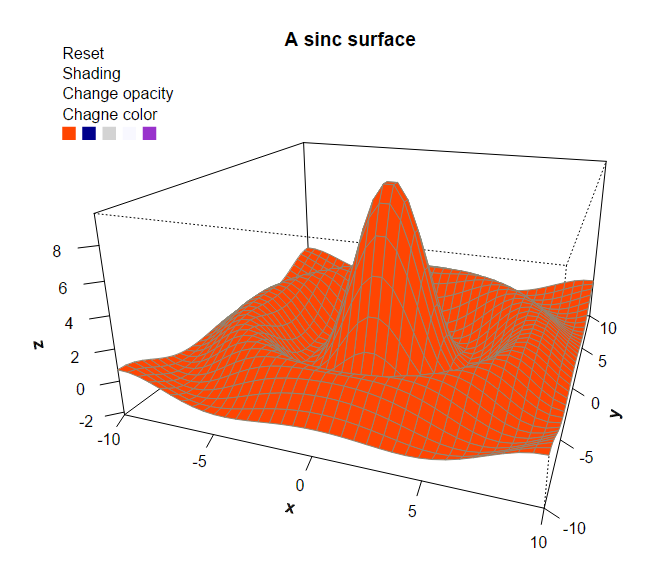
\includegraphics[height = 5cm, width = 5cm]{figure/svg/change_3.PNG}
  \caption{The plot shows the animation that changing the surface color from the left plot to right plot}
  	\label{Example_6.3.1}
\end{center}
\end{figure}

\subsubsection*{Animation of Changing the opacity of the surface}
The figure \ref{Example_6.3.2} shows the opacity of the current sinc surface decreasing during the animation. The middle plot is captured during the duration. 
\begin{figure}[h]
\begin{center}
  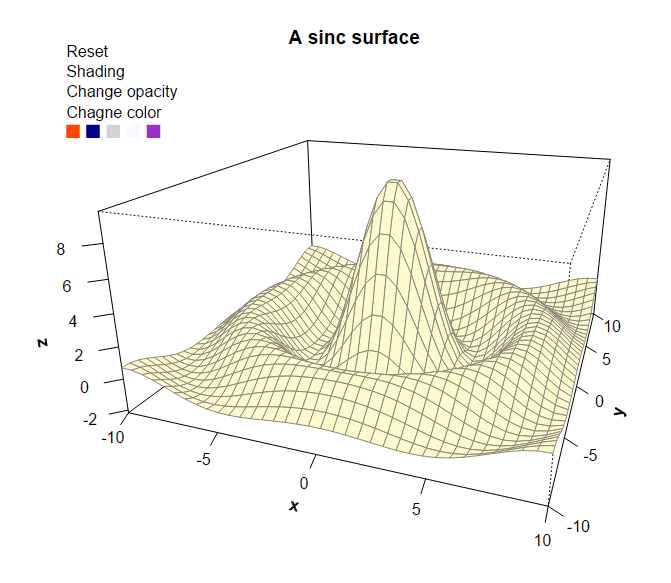
\includegraphics[height = 5cm, width = 5cm]{figure/svg/origin_1.PNG}
  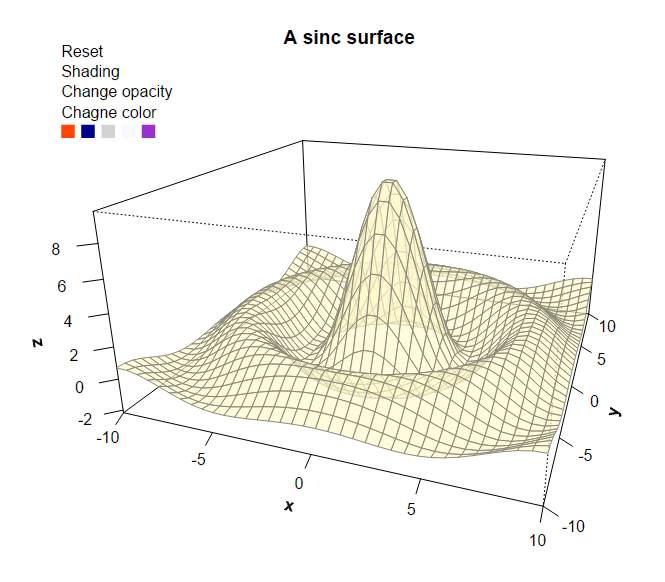
\includegraphics[height = 5cm, width = 5cm]{figure/svg/opacity_2.PNG}
  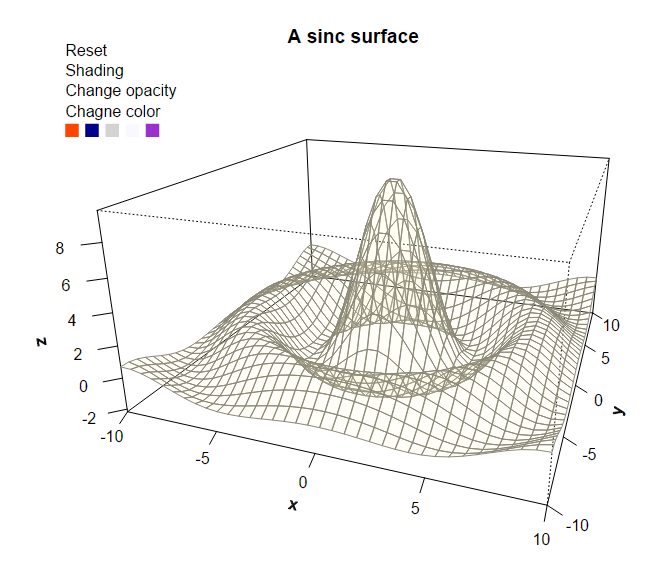
\includegraphics[height = 5cm, width = 5cm]{figure/svg/opacity_3.PNG}
  \caption{The plot shows the animation that decreasing the opacity of sinc surface from the left plot to right plot}
  	\label{Example_6.3.2}
\end{center}
\end{figure}

\subsubsection*{Animation of shading the surface}
The figure \ref{Example_6.3.3} shows the action of adding shade of the current sinc surface. The middle plot is captured during the duration.
\begin{figure}[h]
\begin{center}
  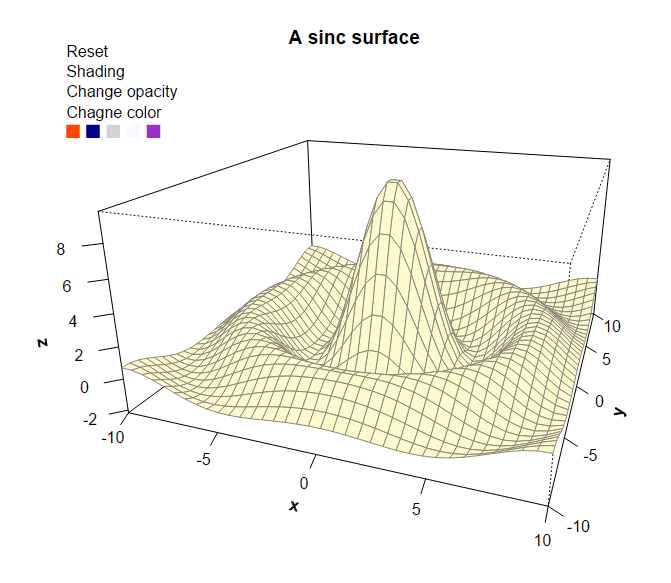
\includegraphics[height = 5cm, width = 5cm]{figure/svg/origin_1.PNG}
  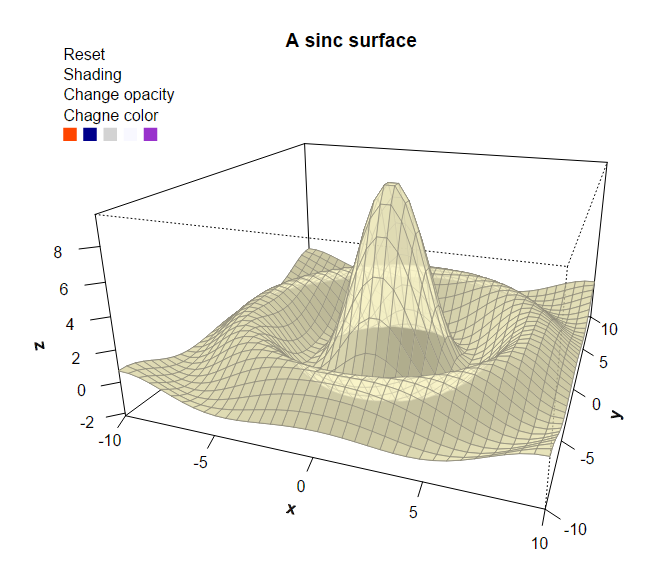
\includegraphics[height = 5cm, width = 5cm]{figure/svg/Shade_2.PNG}
  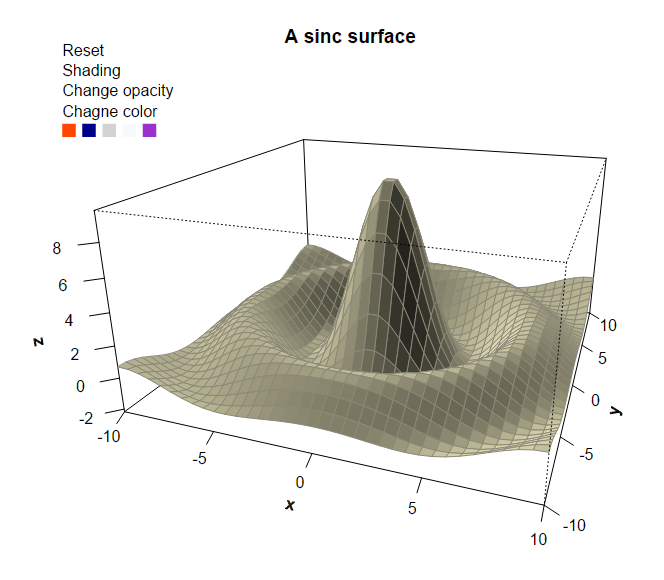
\includegraphics[height = 5cm, width = 5cm]{figure/svg/Shade_3.PNG}
  \caption{The shading animation}
  	\label{Example_6.3.3}
\end{center}
\end{figure}

\subsubsection*{Highlighting the specific fragment of the surface and showing its z-value}
The figure \ref{Example_6.3.4} shows the highlight action. the specific fragment of the sinc surface will been highlightted when the mouse moves into the its area. Also, the z-value of the current selected fragment will be appeared at the top-right region. 
\begin{figure}[h]
\begin{center}
  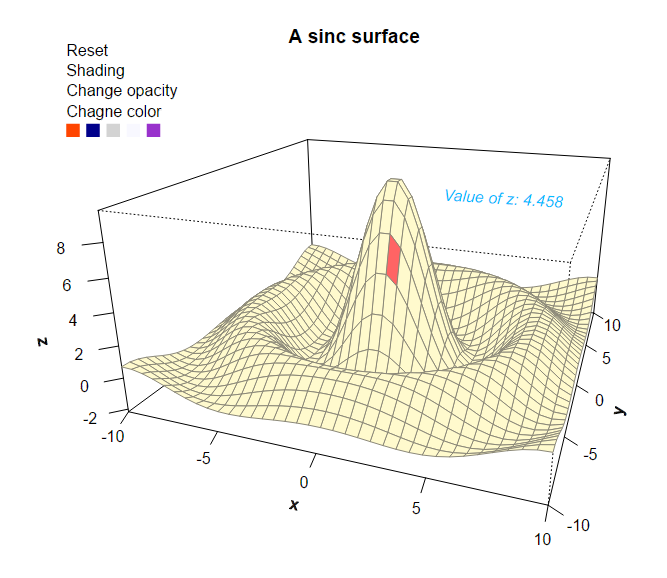
\includegraphics[height = 7.5cm, width = 7.5cm]{figure/svg/hlight_1.PNG}
  \includegraphics[height = 7.5cm, width = 7.5cm]{figure/svg/hlight_2.PNG}
  \caption{The fragment will be highlight when the mouse move into its area. Also its z-value will be appeared}
  	\label{Example_6.3.4}
\end{center}
\end{figure}

\chapter{Conclusion}
\chapter{Reference}
\chapter{Appendix}
\section{persp.R}
\section{filled.contour.R}
\end{document}
